% =====================================================================
%  Paper 2 -- selective edge--cloud plant disease recognition
%  Target: Results in Engineering (Elsevier)
%  Build : latexmk -pdf main.tex   (or upload this folder to Overleaf)
%
%  Every measured value comes from numbers.tex (macros \R...), generated by
%  scripts/make_paper_numbers.py from the hardware run; values not yet
%  measured render as amber "pending" boxes.
%  \note{...} (red) is available for author notes; none remain.
% =====================================================================
\documentclass[preprint,12pt,authoryear]{elsarticle}

\usepackage[T1]{fontenc}
\usepackage{lmodern}
\usepackage{microtype}
\usepackage{amsmath,amssymb}
\usepackage{graphicx}
\usepackage{booktabs}
\usepackage{multirow}
\usepackage{array}
\usepackage{longtable}
\usepackage{xcolor}
\usepackage{tikz}
\usetikzlibrary{positioning,fit,calc,arrows.meta,shapes.geometric,backgrounds}
\usepackage{lineno}
\usepackage[hidelinks]{hyperref}

\definecolor{ink}{HTML}{0B0B0B}\definecolor{inkgray}{HTML}{52514E}
\definecolor{axisgray}{HTML}{C3C2B7}\definecolor{accent}{HTML}{2A78D6}
\definecolor{accentdark}{HTML}{184F95}\definecolor{cloudfill}{HTML}{EEF5FD}
\definecolor{cloudline}{HTML}{86B6EF}\definecolor{edgefill}{HTML}{F5F4F0}
\definecolor{edgeline}{HTML}{C3C2B7}\definecolor{farmA}{HTML}{2A78D6}
\definecolor{farmB}{HTML}{EB6834}\definecolor{farmC}{HTML}{1BAF7A}
\definecolor{farmD}{HTML}{EDA100}
\definecolor{pending}{RGB}{255,228,160}
\definecolor{notecol}{RGB}{176,48,48}
\newcommand{\res}[1]{\colorbox{pending}{\strut\sffamily\footnotesize #1}}
\newcommand{\note}[1]{{\color{notecol}\sffamily\footnotesize[#1]}}
\setlength{\emergencystretch}{2em}
% allow more floats per page so tables/figures stay near their text
\renewcommand{\topfraction}{0.9}\renewcommand{\bottomfraction}{0.8}
\renewcommand{\textfraction}{0.07}\renewcommand{\floatpagefraction}{0.75}
\setcounter{topnumber}{3}\setcounter{totalnumber}{5}
\usepackage{xspace}
% no space between a measured value and a following thin space / unit
\xspaceaddexceptions{\,}
% ragged-right paragraph column for narrow table cells
\newcolumntype{L}[1]{>{\raggedright\arraybackslash}p{#1}}
% Measured values from the embedded run, generated by
% scripts/make_paper_numbers.py (never edit numbers.tex by hand).
% Generated by scripts/make_paper_numbers.py -- do not edit by hand.
% run: results/fleet_run  verify: results/trt_verify_report.json
\newcommand{\RCosMinDinoTwo}{0.9955\xspace}
\newcommand{\RCosMeanDinoTwo}{0.9976\xspace}
\newcommand{\RCosMinDinoThree}{0.9874\xspace}
\newcommand{\RCosMeanDinoThree}{0.9991\xspace}
\newcommand{\RCosMinClip}{0.9474\xspace}
\newcommand{\RCosMeanClip}{0.9911\xspace}
\newcommand{\RMsDinoTwo}{2\,592\xspace}
\newcommand{\RMsDinoThree}{2\,673\xspace}
\newcommand{\RMsClip}{1\,613\xspace}
\newcommand{\RCosMinAll}{0.9474\xspace}
\newcommand{\RAgree}{23/24\xspace}
\newcommand{\RNImg}{3\,677\xspace}
\newcommand{\RNEsc}{684\xspace}
\newcommand{\REscRate}{18.6\,\%\xspace}
\newcommand{\RUpMB}{40.4\xspace}
\newcommand{\RCloudOnlyMB}{216.3\xspace}
\newcommand{\RReduction}{5.4\xspace}
\newcommand{\RKbPerImg}{11.2\,KB\xspace}
\newcommand{\RKbPerImgNum}{11.2\xspace}
\newcommand{\RCloudOnlyKbPerImg}{60.2\xspace}
\newcommand{\RAcc}{76.0\,\%\xspace}
\newcommand{\REdgeAcc}{69.3\,\%\xspace}
\newcommand{\RCloudFail}{0\xspace}
\newcommand{\RMaxPerHour}{14\xspace}
\newcommand{\RAnswerMs}{77\xspace}
\newcommand{\REdgeMs}{70\xspace}
\newcommand{\RNetMs}{69\xspace}
\newcommand{\RCloudS}{6.9\xspace}
\newcommand{\RPayloadKb}{59.5\xspace}
\newcommand{\RDelayMean}{3.5\xspace}
\newcommand{\RDelayMax}{6\xspace}
\newcommand{\RWallMin}{98\xspace}
\newcommand{\RNFlush}{14\xspace}
\newcommand{\RLoadS}{36\xspace}
\newcommand{\RAnswerPNinetyFiveMs}{164\xspace}
\newcommand{\RAnswerEscMs}{139\xspace}
\newcommand{\RVerifierBreakEven}{4.4\xspace}
\newcommand{\RSKb}{60.2\xspace}
\newcommand{\ROffKbOp}{11.2\xspace}
\newcommand{\ROffKbCross}{12.2\xspace}
\newcommand{\ROffKbVer}{20.2\xspace}
\newcommand{\RActDinoTwo}{403\xspace}
\newcommand{\RActDinoThree}{158\,259\xspace}
\newcommand{\RActClip}{225\xspace}
\newcommand{\RActNImg}{64\xspace}
\newcommand{\RNanoRuns}{2\xspace}
\newcommand{\RNanoBatchN}{48\xspace}
\newcommand{\RNanoIdleW}{1.2\xspace}
\newcommand{\RNanoMeanW}{6.3\xspace}
\newcommand{\RNanoMaxW}{7.9\xspace}
\newcommand{\RNanoEImgJ}{49\xspace}
\newcommand{\RNanoEIncrImgJ}{40\xspace}
\newcommand{\RNanoWhPerThousand}{14\xspace}
\newcommand{\RNanoPeakGB}{2.32\xspace}
\newcommand{\RNanoIdleGB}{1.97\xspace}
\newcommand{\RNanoRiseGB}{0.34\xspace}
\newcommand{\RNanoTotalGB}{3.86\xspace}
\newcommand{\RNanoFlushMin}{6.1\xspace}
\newcommand{\RBaseEdgeAcc}{69.3\xspace}
\newcommand{\RBaseTau}{0.138\xspace}
\newcommand{\RBaseEsc}{18.6\xspace}
\newcommand{\RBaseAcc}{75.8\xspace}
\newcommand{\RBasePct}{94.6\xspace}
\newcommand{\RBaseRed}{5.4\xspace}
\newcommand{\RBaseEscNF}{20.3\xspace}
\newcommand{\RKdEdgeAcc}{71.9\xspace}
\newcommand{\RKdTau}{0.072\xspace}
\newcommand{\RKdEsc}{12.3\xspace}
\newcommand{\RKdAcc}{75.4\xspace}
\newcommand{\RKdPct}{94.0\xspace}
\newcommand{\RKdRed}{8.1\xspace}
\newcommand{\RKdEscNF}{15.9\xspace}
\newcommand{\RLoopNWeek}{1\,812\xspace}
\newcommand{\RLoopNEsc}{339\xspace}
\newcommand{\RLoopConfN}{131\xspace}
\newcommand{\RLoopNoneEdge}{69.4\xspace}
\newcommand{\RLoopNoneEsc}{18.7\xspace}
\newcommand{\RLoopReplayEdge}{69.2\xspace}
\newcommand{\RLoopReplayEsc}{20.2\xspace}
\newcommand{\RLoopHardEdge}{68.9\xspace}
\newcommand{\RLoopHardEsc}{21.7\xspace}
\newcommand{\RLoopSoftEdge}{69.3\xspace}
\newcommand{\RLoopSoftEsc}{21.9\xspace}
\newcommand{\RLoopSoftConfEdge}{69.5\xspace}
\newcommand{\RLoopSoftConfEsc}{19.9\xspace}
\newcommand{\RLoopOracleEdge}{68.8\xspace}
\newcommand{\RLoopOracleEsc}{22.3\xspace}
\newcommand{\RPiIdleW}{1.7\xspace}
\newcommand{\RPiLoadW}{3.6\xspace}
\newcommand{\RPiEImgJ}{0.45\xspace}
\newcommand{\RPiEIncrJ}{0.24\xspace}
\newcommand{\RPiN}{300\xspace}
\newcommand{\RSysEJ}{9.5\xspace}
\newcommand{\RSysCloudEJ}{49\xspace}
\newcommand{\RSysERatio}{5.1\xspace}
\newcommand{\RClipSixteenMs}{1\,158\xspace}
\newcommand{\RClipThirtyTwoMs}{1\,613\xspace}
\newcommand{\RClipSixteenLoadS}{10\xspace}
\newcommand{\RClipThirtyTwoLoadS}{19\xspace}
\newcommand{\RClipSixteenCos}{0.9998\xspace}
\newcommand{\RImpNEsc}{455\xspace}
\newcommand{\RImpEscRate}{12.4\,\%\xspace}
\newcommand{\RImpUpMB}{27.0\xspace}
\newcommand{\RImpCloudOnlyMB}{216.3\xspace}
\newcommand{\RImpReduction}{8.0\xspace}
\newcommand{\RImpKbPerImg}{7.5\,KB\xspace}
\newcommand{\RImpAcc}{75.3\,\%\xspace}
\newcommand{\RImpEdgeAcc}{71.9\,\%\xspace}
\newcommand{\RImpCloudFail}{0\xspace}
\newcommand{\RImpAnswerMs}{76\xspace}
\newcommand{\RImpCloudS}{6.5\xspace}
\newcommand{\RImpWallMin}{67\xspace}
\newcommand{\RImpDelayMax}{6\xspace}
\newcommand{\RImpNFlush}{14\xspace}
\newcommand{\RImpLoadS}{33\xspace}
\newcommand{\RImpBatchMed}{34\xspace}
\newcommand{\RImpCloudAgree}{429/455\xspace}
\newcommand{\RImpTau}{0.072\xspace}
\newcommand{\RImpOffEscRate}{12.3\,\%\xspace}
\newcommand{\RNanoTwoEImgJ}{48\xspace}
\newcommand{\RNanoTwoMeanW}{6.9\xspace}
\newcommand{\RNanoTwoFlushMin}{5.6\xspace}
\newcommand{\RNanoTwoPeakGB}{2.10\xspace}
\newcommand{\RImpSysEJ}{6.4\xspace}
\newcommand{\RImpSysERatio}{7.5\xspace}
\newcommand{\RImpFarmAEsc}{11.7\,\%\xspace}
\newcommand{\RImpFarmARed}{8.1\xspace}
\newcommand{\RImpFarmAAcc}{77.8\,\%\xspace}
\newcommand{\RImpFarmBEsc}{19.0\,\%\xspace}
\newcommand{\RImpFarmBRed}{5.3\xspace}
\newcommand{\RImpFarmBAcc}{64.1\,\%\xspace}
\newcommand{\RImpFarmCEsc}{10.9\,\%\xspace}
\newcommand{\RImpFarmCRed}{8.5\xspace}
\newcommand{\RImpFarmCAcc}{75.7\,\%\xspace}
\newcommand{\RImpFarmDEsc}{9.5\,\%\xspace}
\newcommand{\RImpFarmDRed}{11.3\xspace}
\newcommand{\RImpFarmDAcc}{80.1\,\%\xspace}
\newcommand{\RLoadDinoTwoS}{6\xspace}
\newcommand{\RLoadDinoThreeS}{14\xspace}
\newcommand{\RLoadClipS}{17\xspace}
\newcommand{\RBatchMed}{48\xspace}
\newcommand{\RFarmMaxName}{farm~B (solanaceae)\xspace}
\newcommand{\RFarmMaxEsc}{24\,\%\xspace}
\newcommand{\RFarmMinName}{farm~D (market garden)\xspace}
\newcommand{\RFarmMinEsc}{15\,\%\xspace}
\newcommand{\RImgPerDay}{100\xspace}
\newcommand{\RMonthMB}{33\xspace}
\newcommand{\RMonthCloudMB}{177\xspace}
\newcommand{\RUplinkMbps}{1\xspace}
\newcommand{\RUplinkS}{0.5\xspace}
\newcommand{\RCloudAgreeFleet}{652/684\xspace}
\newcommand{\RCloudAgreeFleetPct}{95.3\,\%\xspace}
\newcommand{\RCloudAccEsc}{67.4\,\%\xspace}
\newcommand{\ROfflineCloudAccEsc}{66.5\,\%\xspace}
\newcommand{\REngCosMinDinoTwo}{0.9965\xspace}
\newcommand{\REngCosMeanDinoTwo}{0.9979\xspace}
\newcommand{\REngCosMinDinoThree}{1.0000\xspace}
\newcommand{\REngCosMeanDinoThree}{1.0000\xspace}
\newcommand{\REngCosMinClip}{1.0000\xspace}
\newcommand{\REngCosMeanClip}{1.0000\xspace}
\newcommand{\REngAgree}{24/24\xspace}
\newcommand{\RFarmAEsc}{18.9\,\%\xspace}
\newcommand{\RFarmAUp}{14.6\xspace}
\newcommand{\RFarmACloud}{75.3\xspace}
\newcommand{\RFarmARed}{5.1\xspace}
\newcommand{\RFarmAAcc}{79.9\,\%\xspace}
\newcommand{\RFarmAEdgeAcc}{72.3\,\%\xspace}
\newcommand{\RFarmBEsc}{23.8\,\%\xspace}
\newcommand{\RFarmBUp}{9.4\xspace}
\newcommand{\RFarmBCloud}{38.9\xspace}
\newcommand{\RFarmBRed}{4.1\xspace}
\newcommand{\RFarmBAcc}{62.2\,\%\xspace}
\newcommand{\RFarmBEdgeAcc}{56.5\,\%\xspace}
\newcommand{\RFarmCEsc}{17.8\,\%\xspace}
\newcommand{\RFarmCUp}{7.7\xspace}
\newcommand{\RFarmCCloud}{43.6\xspace}
\newcommand{\RFarmCRed}{5.6\xspace}
\newcommand{\RFarmCAcc}{75.1\,\%\xspace}
\newcommand{\RFarmCEdgeAcc}{69.3\,\%\xspace}
\newcommand{\RFarmDEsc}{14.7\,\%\xspace}
\newcommand{\RFarmDUp}{8.6\xspace}
\newcommand{\RFarmDCloud}{58.6\xspace}
\newcommand{\RFarmDRed}{6.8\xspace}
\newcommand{\RFarmDAcc}{81.6\,\%\xspace}
\newcommand{\RFarmDEdgeAcc}{74.8\,\%\xspace}
\newcommand{\RImpMonthMB}{22\xspace}
\newcommand{\REscNFSmall}{43.5\xspace}
\newcommand{\RAccNFSmall}{76.18\xspace}
\newcommand{\RPctNFSmall}{95.0\xspace}
\newcommand{\REdgeAccSmall}{61.08\xspace}
\newcommand{\REscNFLarge}{20.3\xspace}
\newcommand{\RAccNFLarge}{76.18\xspace}
\newcommand{\RPctNFLarge}{95.0\xspace}
\newcommand{\REdgeAccLarge}{69.32\xspace}
\newcommand{\REscNFEff}{21.4\xspace}
\newcommand{\RAccNFEff}{76.18\xspace}
\newcommand{\RPctNFEff}{95.0\xspace}
\newcommand{\REdgeAccEff}{69.35\xspace}
\newcommand{\REscNFKd}{15.9\xspace}
\newcommand{\RAccNFKd}{76.18\xspace}
\newcommand{\RPctNFKd}{95.0\xspace}
\newcommand{\REdgeAccKd}{71.91\xspace}
\newcommand{\RVerEscNF}{29.0\xspace}
\newcommand{\RVerAccNF}{76.18\xspace}
\newcommand{\RVerAuc}{0.731\xspace}
\newcommand{\RVerValAuc}{0.848\xspace}
\newcommand{\RVerExtra}{8.8\xspace}
\newcommand{\RBudFiveMaxP}{71.72\xspace}
\newcommand{\RBudFiveMargin}{71.34\xspace}
\newcommand{\RBudFiveEnt}{71.50\xspace}
\newcommand{\RBudFiveOracle}{74.33\xspace}
\newcommand{\RBudTenMaxP}{73.43\xspace}
\newcommand{\RBudTenMargin}{73.27\xspace}
\newcommand{\RBudTenEnt}{73.21\xspace}
\newcommand{\RBudTenOracle}{79.33\xspace}
\newcommand{\RBudFifteenMaxP}{74.79\xspace}
\newcommand{\RBudFifteenMargin}{74.82\xspace}
\newcommand{\RBudFifteenEnt}{74.84\xspace}
\newcommand{\RBudFifteenOracle}{84.34\xspace}
\newcommand{\RBudTwentyMaxP}{76.09\xspace}
\newcommand{\RBudTwentyMargin}{76.09\xspace}
\newcommand{\RBudTwentyEnt}{75.80\xspace}
\newcommand{\RBudTwentyOracle}{84.80\xspace}
\newcommand{\RBudTwentyFiveMaxP}{77.21\xspace}
\newcommand{\RBudTwentyFiveMargin}{77.10\xspace}
\newcommand{\RBudTwentyFiveEnt}{76.67\xspace}
\newcommand{\RBudTwentyFiveOracle}{84.80\xspace}
\newcommand{\RBudThirtyMaxP}{78.00\xspace}
\newcommand{\RBudThirtyMargin}{78.00\xspace}
\newcommand{\RBudThirtyEnt}{77.45\xspace}
\newcommand{\RBudThirtyOracle}{84.80\xspace}
\newcommand{\RBudSpread}{0.5\xspace}
\newcommand{\RGapClosedThirty}{80\xspace}
\newcommand{\RTemp}{0.84\xspace}
\newcommand{\REceRaw}{0.097\xspace}
\newcommand{\REceScaled}{0.054\xspace}
\newcommand{\RSigMarginAuc}{0.810\xspace}
\newcommand{\RSigMarginEsc}{20.3\xspace}
\newcommand{\RSigMarginTAuc}{0.811\xspace}
\newcommand{\RSigMarginTEsc}{20.7\xspace}
\newcommand{\RSigMaxPAuc}{0.806\xspace}
\newcommand{\RSigMaxPEsc}{20.4\xspace}
\newcommand{\RSigMaxPTAuc}{0.810\xspace}
\newcommand{\RSigMaxPTEsc}{20.2\xspace}
\newcommand{\RSigEntAuc}{0.790\xspace}
\newcommand{\RSigEntEsc}{22.7\xspace}
\newcommand{\RSigEntTAuc}{0.797\xspace}
\newcommand{\RSigEntTEsc}{21.2\xspace}
\newcommand{\RSigLogitAuc}{0.810\xspace}
\newcommand{\RSigLogitEsc}{21.5\xspace}
\newcommand{\RTempKd}{0.74\xspace}
\newcommand{\REceKdRaw}{0.125\xspace}
\newcommand{\REceKdScaled}{0.038\xspace}
\newcommand{\RSigKdMarginAuc}{0.830\xspace}
\newcommand{\RSigKdMarginEsc}{15.9\xspace}
\newcommand{\RSigKdMarginTAuc}{0.829\xspace}
\newcommand{\RSigKdMarginTEsc}{16.6\xspace}
\newcommand{\RSigKdMaxPAuc}{0.823\xspace}
\newcommand{\RSigKdMaxPEsc}{14.5\xspace}
\newcommand{\RSigKdMaxPTAuc}{0.829\xspace}
\newcommand{\RSigKdMaxPTEsc}{15.6\xspace}
\newcommand{\RSigKdEntAuc}{0.797\xspace}
\newcommand{\RSigKdEntEsc}{15.7\xspace}
\newcommand{\RSigKdEntTAuc}{0.814\xspace}
\newcommand{\RSigKdEntTEsc}{14.8\xspace}
\newcommand{\RSigKdLogitAuc}{0.821\xspace}
\newcommand{\RSigKdLogitEsc}{17.3\xspace}
\newcommand{\RBootPctLo}{92.1\xspace}
\newcommand{\RBootPctMed}{94.6\xspace}
\newcommand{\RBootPctHi}{96.0\xspace}
\newcommand{\RBootEscLo}{12.3\xspace}
\newcommand{\RBootEscHi}{23.5\xspace}
\newcommand{\RBootShare}{28\xspace}
\newcommand{\RConsTau}{0.198\xspace}
\newcommand{\RConsEsc}{23.5\xspace}
\newcommand{\RConsPct}{96.0\xspace}
\newcommand{\RConsRed}{4.3\xspace}
\newcommand{\RBootKdPctLo}{92.3\xspace}
\newcommand{\RBootKdPctMed}{94.0\xspace}
\newcommand{\RBootKdPctHi}{96.0\xspace}
\newcommand{\RBootKdEscLo}{7.5\xspace}
\newcommand{\RBootKdEscHi}{20.0\xspace}
\newcommand{\RBootKdShare}{20\xspace}
\newcommand{\RConsKdTau}{0.138\xspace}
\newcommand{\RConsKdEsc}{20.0\xspace}
\newcommand{\RConsKdPct}{96.0\xspace}
\newcommand{\RConsKdRed}{5.0\xspace}
\newcommand{\RIsoEsc}{14.3\xspace}
\newcommand{\RIsoRed}{7.0\xspace}
\newcommand{\RIsoRunEsc}{15.3\xspace}
\newcommand{\RIsoRunRed}{6.5\xspace}
\newcommand{\RMfEdge}{65.8\xspace}
\newcommand{\RMfOp}{72.9\xspace}
\newcommand{\RMfCloud}{77.5\xspace}
\newcommand{\RMfKdEdge}{68.6\xspace}
\newcommand{\RMfKdOp}{72.6\xspace}
\newcommand{\RMfRunOne}{73.2\xspace}
\newcommand{\RMfRunTwo}{72.6\xspace}
\newcommand{\RFarmACeil}{84.3\,\%\xspace}
\newcommand{\RFarmAPctCloud}{94.8\,\%\xspace}
\newcommand{\RFarmBCeil}{66.3\,\%\xspace}
\newcommand{\RFarmBPctCloud}{93.8\,\%\xspace}
\newcommand{\RFarmCCeil}{80.1\,\%\xspace}
\newcommand{\RFarmCPctCloud}{93.8\,\%\xspace}
\newcommand{\RFarmDCeil}{84.8\,\%\xspace}
\newcommand{\RFarmDPctCloud}{96.2\,\%\xspace}
\newcommand{\RImpFarmACeil}{84.3\,\%\xspace}
\newcommand{\RImpFarmAPctCloud}{92.3\,\%\xspace}
\newcommand{\RImpFarmBCeil}{66.3\,\%\xspace}
\newcommand{\RImpFarmBPctCloud}{96.6\,\%\xspace}
\newcommand{\RImpFarmCCeil}{80.1\,\%\xspace}
\newcommand{\RImpFarmCPctCloud}{94.5\,\%\xspace}
\newcommand{\RImpFarmDCeil}{84.8\,\%\xspace}
\newcommand{\RImpFarmDPctCloud}{94.4\,\%\xspace}
\newcommand{\RTrtChunkSixteenMB}{147\xspace}
\newcommand{\RTrtChunkThirtyTwoMB}{294\xspace}
\newcommand{\RTrtDiskGB}{2.87\xspace}
\newcommand{\RNanoRiseSixteenGB}{0.22\xspace}
\newcommand{\RNanoRiseThirtyTwoGB}{0.46\xspace}
\newcommand{\RAnswerLocalMs}{74\xspace}
\newcommand{\RNanoThreeFourN}{34\xspace}
\newcommand{\RNanoThreeFourRuns}{3\xspace}
\newcommand{\RNanoThreeFourEImgJ}{48\xspace}
\newcommand{\RImpSysEThreeFourJ}{6.4\xspace}
\newcommand{\RImpSysEFpThirtyTwoJ}{6.5\xspace}
\newcommand{\RRouterEsc}{41.3\xspace}
\newcommand{\RRouterDinoEsc}{42.0\xspace}
\newcommand{\RRouterAuc}{0.785\xspace}
\newcommand{\RRouterDinoAuc}{0.768\xspace}
\newcommand{\RSmallAucLo}{0.76\xspace}
\newcommand{\RSmallAucHi}{0.79\xspace}
\newcommand{\RRefEscFullAcc}{66.8\,\%\xspace}
\newcommand{\RRefEscPayAcc}{68.1\,\%\xspace}
\newcommand{\RPayNanoAgree}{662/684\xspace}
\newcommand{\RPayN}{1\,820\xspace}
\newcommand{\RPayOrigKb}{148.9\xspace}
\newcommand{\RPayOrigAcc}{79.6\,\%\xspace}
\newcommand{\RPayOrigAgree}{100.0\,\%\xspace}
\newcommand{\RPayFullKb}{133.2\xspace}
\newcommand{\RPayFullAcc}{79.8\,\%\xspace}
\newcommand{\RPayFullAgree}{99.2\,\%\xspace}
\newcommand{\RPayFourFourEightKb}{59.1\xspace}
\newcommand{\RPayFourFourEightAcc}{79.8\,\%\xspace}
\newcommand{\RPayFourFourEightAgree}{98.4\,\%\xspace}
\newcommand{\RPayThreeThreeSixQNinetyFiveKb}{57.1\xspace}
\newcommand{\RPayThreeThreeSixQNinetyFiveAcc}{79.6\,\%\xspace}
\newcommand{\RPayThreeThreeSixQNinetyFiveAgree}{98.1\,\%\xspace}
\newcommand{\RPayThreeThreeSixKb}{41.9\xspace}
\newcommand{\RPayThreeThreeSixAcc}{79.3\,\%\xspace}
\newcommand{\RPayThreeThreeSixAgree}{97.8\,\%\xspace}
\newcommand{\RPayTwoTwoFourKb}{22.9\xspace}
\newcommand{\RPayTwoTwoFourAcc}{78.8\,\%\xspace}
\newcommand{\RPayTwoTwoFourAgree}{95.4\,\%\xspace}
\newcommand{\RPayRatio}{2.3\xspace}
\newcommand{\RLoopParts}{5\xspace}
\newcommand{\RLoopNoneEdgeSd}{0.5\xspace}
\newcommand{\RLoopNoneEscSd}{2.1\xspace}
\newcommand{\RLoopNoneEscTau}{18.4\xspace}
\newcommand{\RLoopNoneEscTauSd}{0.6\xspace}
\newcommand{\RLoopNoneAccTau}{76.0\xspace}
\newcommand{\RLoopNoneAccTauSd}{0.7\xspace}
\newcommand{\RLoopNonePct}{94.9\xspace}
\newcommand{\RLoopNoneRed}{5.4\xspace}
\newcommand{\RLoopReplayEdgeSd}{0.5\xspace}
\newcommand{\RLoopReplayEscSd}{1.9\xspace}
\newcommand{\RLoopReplayEscTau}{20.1\xspace}
\newcommand{\RLoopReplayEscTauSd}{0.6\xspace}
\newcommand{\RLoopReplayAccTau}{76.2\xspace}
\newcommand{\RLoopReplayAccTauSd}{0.5\xspace}
\newcommand{\RLoopReplayPct}{95.2\xspace}
\newcommand{\RLoopReplayRed}{5.0\xspace}
\newcommand{\RLoopHardEdgeSd}{0.9\xspace}
\newcommand{\RLoopHardEscSd}{2.7\xspace}
\newcommand{\RLoopHardEscTau}{17.1\xspace}
\newcommand{\RLoopHardEscTauSd}{1.1\xspace}
\newcommand{\RLoopHardAccTau}{74.9\xspace}
\newcommand{\RLoopHardAccTauSd}{0.9\xspace}
\newcommand{\RLoopHardPct}{93.6\xspace}
\newcommand{\RLoopHardRed}{5.9\xspace}
\newcommand{\RLoopSoftEdgeSd}{0.8\xspace}
\newcommand{\RLoopSoftEscSd}{2.6\xspace}
\newcommand{\RLoopSoftEscTau}{18.6\xspace}
\newcommand{\RLoopSoftEscTauSd}{0.7\xspace}
\newcommand{\RLoopSoftAccTau}{75.4\xspace}
\newcommand{\RLoopSoftAccTauSd}{0.9\xspace}
\newcommand{\RLoopSoftPct}{94.2\xspace}
\newcommand{\RLoopSoftRed}{5.4\xspace}
\newcommand{\RLoopSoftConfEdgeSd}{0.6\xspace}
\newcommand{\RLoopSoftConfEscSd}{2.3\xspace}
\newcommand{\RLoopSoftConfEscTau}{18.5\xspace}
\newcommand{\RLoopSoftConfEscTauSd}{1.1\xspace}
\newcommand{\RLoopSoftConfAccTau}{75.8\xspace}
\newcommand{\RLoopSoftConfAccTauSd}{0.6\xspace}
\newcommand{\RLoopSoftConfPct}{94.7\xspace}
\newcommand{\RLoopSoftConfRed}{5.4\xspace}
\newcommand{\RLoopOracleEdgeSd}{0.6\xspace}
\newcommand{\RLoopOracleEscSd}{2.5\xspace}
\newcommand{\RLoopOracleEscTau}{17.5\xspace}
\newcommand{\RLoopOracleEscTauSd}{0.3\xspace}
\newcommand{\RLoopOracleAccTau}{74.8\xspace}
\newcommand{\RLoopOracleAccTauSd}{0.9\xspace}
\newcommand{\RLoopOraclePct}{93.4\xspace}
\newcommand{\RLoopOracleRed}{5.7\xspace}
\newcommand{\RLoopCtlVsNone}{+1.5\xspace}
\newcommand{\RLoopCtlVsNoneSd}{0.5\xspace}
\newcommand{\RLoopHardVsCtl}{+1.4\xspace}
\newcommand{\RLoopHardVsCtlSd}{1.9\xspace}
\newcommand{\RLoopSoftVsCtl}{+1.7\xspace}
\newcommand{\RLoopSoftVsCtlSd}{2.3\xspace}
\newcommand{\RLoopSoftConfVsCtl}{-0.3\xspace}
\newcommand{\RLoopSoftConfVsCtlSd}{1.6\xspace}
\newcommand{\RLoopOracleVsCtl}{+2.1\xspace}
\newcommand{\RLoopOracleVsCtlSd}{3.1\xspace}


\journal{Results in Engineering}

\begin{document}

\begin{frontmatter}

\title{Diagnose locally, escalate rarely: bandwidth-efficient plant disease
recognition with foundation models on embedded edge--cloud \mbox{hardware}}
% Alternative titles:
%  - Selective edge--cloud inference for in-the-wild plant disease diagnosis:
%    a bandwidth-centred evaluation on embedded hardware
%  - Less uplink, same diagnosis: margin-based escalation from a Raspberry Pi
%    to a foundation-model ensemble on a Jetson Nano

\author[uit2]{Youssef Natij\corref{cor1}}
\ead{youssef.natij@uit.ac.ma}
\author[uit1]{Hajar El Karch}
\ead{hajar.elkarch@uit.ac.ma}
\author[uit2]{Abdelkader Mezouari}
\ead{abdelkader.mezouari1@uit.ac.ma}
\cortext[cor1]{Corresponding author.}

\affiliation[uit2]{organization={Scientific Research and Innovation Laboratory, Higher School of Technology, Ibn Tofail University},
  addressline={Campus Universitaire, B.P. 242}, postcode={14000}, city={Kenitra}, country={Morocco}}
\affiliation[uit1]{organization={Laboratory of Advanced Systems Engineering, National School of Applied Engineering, Ibn Tofail University},
  addressline={Campus Universitaire, B.P. 241}, postcode={14000}, city={Kenitra}, country={Morocco}}

\begin{abstract}
Image-based plant disease diagnosis in the field faces a dilemma:
lightweight models run on low-cost farm devices but misdiagnose about one
field photograph in three, whereas foundation-model ensembles approach
expert accuracy but need every photograph uploaded over weak, metered
rural links. We study selective edge--cloud inference as the middle
ground, evaluated by uplink traffic, the binding constraint on farms. On
PlantWild (18\,542 in-the-wild images, 89
classes), a MobileNetV3-Large edge classifier escalates an image to a
three-backbone foundation-model ensemble only when its two most probable
classes are closer than a validation-calibrated threshold. The rule escalates 18.6\,\% of test images and retains
94.6\,\% of always-cloud accuracy, cutting uplink traffic 5.4-fold. Edge-model capacity, not router
sophistication, sets this operating point: a weaker edge model needs
\REscNFSmall\,\% escalation for the same target, and a cloud-supervised verifier
ranks useful escalations worse than the margin (AUC 0.731 vs.\ 0.810) and
adds an always-on message. We deploy the system on a Raspberry Pi~5 and
an end-of-life 4\,GB Jetson Nano, porting the ensemble to
framework-free, chunk-by-chunk TensorRT inference. In an emulated
seven-day, four-farm deployment, it uploads
\RReduction{}$\times$ less than always-cloud, answers on the farm in
\RAnswerMs\,ms (median) and confirms each escalated image with \RCloudS\,s
of Nano compute. Distilling the ensemble into the same edge model, at no
cost on the device, raises the measured saving to
\RImpReduction{}$\times$ and cuts device energy per diagnosis by a third.
Selective escalation thus brings foundation-model accuracy to rural
links on commodity hardware.
\end{abstract}

\begin{highlights}
\item An edge model escalates only uncertain field images to a foundation-model ensemble
\item 18.6\,\% escalation retains 94.6\,\% of cloud accuracy with 5.4$\times$ less uplink
\item Edge-model capacity, not router complexity, sets the trade-off
\item A 0.9-billion-parameter ensemble runs on an end-of-life 4\,GB Jetson Nano
\item Four-farm emulation on the devices: 5.4$\times$ less uplink, 8$\times$ with a distilled edge
\end{highlights}

\begin{keyword}
plant disease recognition \sep edge computing \sep selective inference
\sep foundation models \sep bandwidth efficiency \sep embedded systems
\end{keyword}

\end{frontmatter}

\linenumbers

% =====================================================================
\section{Introduction}
\label{sec:intro}
% =====================================================================

Pathogens and pests destroy a substantial fraction of the global harvest
of major food crops every year \citep{savary2019global}, and early,
accurate diagnosis is what allows a grower to respond before an outbreak
spreads. Smartphone and camera-based diagnosis has therefore become one
of the most studied applications of deep learning in agriculture
\citep{kamilaris2018survey, mohanty2016deeplearning,
ferentinos2018deep}. Yet the field has long been flattered by
laboratory benchmarks: models that exceed 99\,\% accuracy on curated
leaf images such as PlantVillage \citep{hughes2015plantvillage} lose much
of that accuracy on photographs taken in real fields, where backgrounds
are cluttered, lighting is uncontrolled and symptoms are small
\citep{barbedo2018impact, noyan2022uncovering, ahmad2023toward,
wu2023fromlaboratoryto}. The PlantWild benchmark \citep{wei2024plantwild}
made this gap measurable at scale, with 18\,542 in-the-wild images
spanning 89 crop--disease classes.

Two families of models now address this setting, and they sit at
opposite ends of a deployment trade-off. Frozen \emph{foundation-model}
features --- self-supervised DINOv2 and DINOv3 and language-supervised
CLIP \citep{oquab2024dinov2, simeoni2025dinov3, radford2021clip} --- are
remarkably robust to field conditions; in prior work we showed that
fusing three such backbones reaches 80.17\,\% top-1 on PlantWild without
any text supervision \citep{elkarch2026backbone}. Such ensembles,
however, total close to a billion parameters and must run on a server.
Lightweight convolutional networks such as MobileNetV3
\citep{howard2019mobilenetv3} run comfortably on a farm-grade device but
fall more than ten points short in the wild. A grower must thus choose
between an accurate model that requires connectivity and a local model
that is frequently wrong.

Connectivity is precisely what rural agriculture lacks. Cellular uplinks
on farms are slow, intermittent and metered \citep{wolfert2017bigdata,
ogrady2019edge}, and every photograph sent to a server costs airtime,
energy and money. Uploading every image is the most expensive way to use
a scarce resource, yet it is the implicit assumption of most cloud-based
diagnosis systems. Edge computing \citep{shi2016edge} suggests the
alternative: process data where it is produced and send only what
cannot be handled locally.

This paper studies \emph{selective escalation}: an edge model diagnoses
every image locally and forwards an image to the cloud ensemble only
when it is uncertain. The idea is old in machine learning ---
classifier cascades \citep{viola2001cascade}, the reject option
\citep{chow1970reject} and early exiting \citep{teerapittayanon2016branchynet}
all exploit it --- but its evaluation has centred on computation and
latency. For connected agriculture the binding constraint is the uplink,
so we make \emph{bytes uploaded per diagnosis} the primary cost axis and
ask three questions:
\begin{enumerate}
\item How much uplink traffic can selective escalation save while
      retaining most of the cloud ensemble's accuracy on in-the-wild images?
\item What determines the achievable operating point: the edge model, or
      the sophistication of the escalation rule?
\item Does the approach survive contact with real embedded hardware,
      including a cloud node small enough to sit on a farm or in a
      cooperative?
\end{enumerate}

\paragraph{Contributions}
\begin{itemize}
\item \textbf{A bandwidth-centred evaluation of selective edge--cloud
      inference for plant disease recognition.} A MobileNetV3-Large edge
      model with a one-line margin rule, its threshold calibrated on
      validation data, retains 94.6\,\% of the ensemble's accuracy on held-out
      test images while escalating 18.6\,\% of them, a 5.4-fold reduction in
      uplink traffic (Section~\ref{sec:res-headline}).
\item \textbf{Evidence that edge capacity, not router cleverness, sets the
      operating point.} Upgrading the edge model halves the required
      escalation rate (\REscNFSmall\,\% $\rightarrow$ \REscNFLarge\,\%), and distilling the
      ensemble into the same edge model --- once, before deployment, with
      no change on the device --- raises the uplink saving measured on the
      devices from \RReduction- to \RImpReduction-fold, and from
      \RBaseRed- to \RIsoRed-fold at equal accuracy, whereas a
      learned edge-side router saves only two points of escalation and a
      cloud-supervised verifier does worse than the scalar margin while
      adding a permanent message overhead
      (Sections~\ref{sec:res-capacity}--\ref{sec:res-teacher}
      and~\ref{sec:res-improved}).
\item \textbf{A recipe for running foundation models on end-of-life
      embedded hardware.} The edge runs on a Raspberry Pi~5, and the
      0.9-billion-parameter ensemble runs on a 4\,GB Jetson Nano whose last
      software release predates every framework the ensemble needs. Five
      principles make this possible --- decoupling the model from its
      framework, compiling within the memory ceiling, choosing precision
      by measurement, chunk-major batched inference and stage-by-stage
      verification --- and the board serves an escalated image with
      \RNanoEImgJ\,J of energy, with board memory peaking at
      \RNanoPeakGB\,GB
      (Section~\ref{sec:port} and \mbox{\ref{app:adaptations}}).
\item \textbf{A trace-driven, hardware-in-the-loop emulation of a
      multi-farm week.} Four virtual farms with distinct crop portfolios
      play back a seven-day capture schedule on the real devices, yielding
      measured per-image latency, per-farm upload volume, cloud load and
            device energy, for the original and the distilled edge model
      (Sections~\ref{sec:res-fleet} and~\ref{sec:res-improved}).
\end{itemize}

% =====================================================================
\section{Related work}
\label{sec:related}
% =====================================================================

\subsection{Plant disease recognition in the wild}
\label{sec:rel-plant}
Early deep-learning studies reported near-perfect accuracy on
laboratory images \citep{mohanty2016deeplearning, ferentinos2018deep},
but subsequent work traced much of that performance to dataset bias and
showed sharp drops under field conditions \citep{barbedo2018impact,
noyan2022uncovering, ahmad2023toward}. Field-oriented datasets such as
PlantDoc \citep{singh2020plantdoc} and, at a larger scale, PlantWild
\citep{wei2024plantwild} now drive the area, together with multimodal
baselines that inject textual disease descriptions
\citep{wei2024mvpdr}. Recent work combines foundation backbones
\citep{jiang2025plantcafo, salman2025plantdisease} or compresses ensembles
for deployment \citep{hasan2025deployable}. Our cloud model is the
three-backbone QualityGate fusion of \citet{elkarch2026backbone}; this
paper does not propose a new recogniser but asks how to deliver such a
recogniser's accuracy to farms that cannot afford to upload every image.

\subsection{Edge--cloud collaborative inference}
Collaborative inference distributes a model's computation between a
device and a server. Neurosurgeon partitions a single network at the
layer that minimises latency or energy \citep{kang2017neurosurgeon};
distributed DNNs and early-exit networks attach classifiers to
intermediate layers so that easy inputs leave early
\citep{teerapittayanon2016branchynet, teerapittayanon2017ddnn}; split
computing compresses the intermediate tensor sent over the network
\citep{matsubara2022split}. These methods co-design a single model. We
study the complementary \emph{model-cascade} setting, in which the edge
and cloud models are independent and the cloud model is a frozen
ensemble that cannot be partitioned or retrained for the edge --- the
practical situation when the best available recogniser is a set of
foundation backbones.

\subsection{Cascades, selective prediction and escalation rules}
Deciding which inputs deserve the expensive model is a selective
prediction problem \citep{chow1970reject, geifman2017selective}. The
maximum softmax probability is a strong baseline for detecting likely
errors \citep{hendrycks2017baseline}, although modern networks are
miscalibrated \citep{guo2017calibration}. Learned deferral policies
have been proposed for cascades \citep{wang2018idk} and for edge devices
that query a cloud model \citep{kag2023selective}. We compare scalar
uncertainty signals against both edge-side learned routers and a
cloud-supervised verifier, and we account for the bandwidth that a
learned verifier itself consumes --- a cost that latency-centred
evaluations omit.

\subsection{Edge AI in agriculture}
Surveys of deep learning in agriculture \citep{kamilaris2018survey} and
of smart farming \citep{wolfert2017bigdata} identify connectivity and
on-farm computation as recurring obstacles, and edge computing has been
argued to be a natural fit for agricultural data
\citep{ogrady2019edge}. The disease-recognition studies discussed in
Section~\ref{sec:rel-plant}, however, evaluate either a server-side or a
fully on-device classifier and report accuracy and, at most,
computational cost; none of them measures the uplink traffic that a
deployment would generate. Our deployment also differs in placing the large model on an
embedded node rather than in a data centre.

% =====================================================================
\section{Materials and methods}
\label{sec:methods}
% =====================================================================

\subsection{Dataset and protocol}
\label{sec:data}
We use PlantWild \citep{wei2024plantwild}: 18\,542 field photographs of
89 classes spanning healthy and diseased leaves of more than thirty plant
species. We follow the official split procedure of
\citet{wei2024mvpdr} (fixed seed, 80\,\% train-validation and 20\,\%
test, with 12.5\,\% of train-validation held out for validation),
giving 13\,045 training, 1\,820 validation and 3\,677 test images. All
accuracies are top-1 on the 3\,677-image test split. Training, offline
evaluation and the ONNX export ran on a workstation with an NVIDIA
GeForce RTX~3070 (8\,GB), an AMD Ryzen~7 7700 CPU and 64\,GB of RAM.

\subsection{Cloud model: frozen foundation-backbone fusion}
\label{sec:cloud}
The cloud model is the QualityGate fusion of \citet{elkarch2026backbone}
(Fig.~\ref{fig:system}, right). Three frozen backbones each produce a
global image descriptor: DINOv2 ViT-L/14 at 336\,px
\citep{oquab2024dinov2}, DINOv3 ViT-L/16 at 336\,px
\citep{simeoni2025dinov3}, and the CLIP ViT-L/14 image encoder at
224\,px \citep{radford2021clip}. Each descriptor is
$\ell_2$-normalised, the three are concatenated into a 2\,816-dimensional
vector and the result is normalised again, giving $\hat{x}$. The
QualityGate head mixes a linear classifier with a prototype classifier
($K{=}8$ prototypes $p_{c,k}$ per class) through a learned per-class gate:
\begin{equation}
z_c = g_c \left(w_c^\top \hat{x} + b_c\right)
      + (1 - g_c)\,\frac{1}{T}\max_{k}\,\cos\!\left(\hat{x}, p_{c,k}\right),
\qquad g_c = \sigma(\gamma_c),
\label{eq:qg}
\end{equation}
with a learned temperature $T$. Only the head is trained (2.3\,M
parameters, 50 epochs); the backbones total about 0.9\,B frozen
parameters. The model reaches 80.17\,\% top-1 and 77.49\,\% macro-F1 on
the test split, and we refer to it as \emph{always-cloud}.

\subsection{Edge models}
\label{sec:edge}
We consider three ImageNet-pretrained convolutional networks that fit a
farm-grade CPU:
MobileNetV3-Small, MobileNetV3-Large \citep{howard2019mobilenetv3} and
EfficientNet-B0 \citep{tan2019efficientnet}. Each is fine-tuned end to
end at $224{\times}224$ for 30 epochs with AdamW
\citep{loshchilov2019adamw} (learning rate $5{\times}10^{-4}$, weight decay
$10^{-4}$, batch 64, cosine schedule with 5\,\% linear warm-up), focal
loss \citep{lin2017focal} with $\gamma{=}2$ and label smoothing 0.1, and
random resized crops (scale 0.6--1.0), horizontal flips and colour
jitter. The models are trained on 11\,778 of the 13\,045 training images; the
remaining 1\,267 (10\,\% of each class, rounded down) select the
checkpoint with the best macro-F1, so that the 1\,820 validation images
remain unseen until the escalation threshold is calibrated on them.

\subsection{Margin-based escalation}
\label{sec:router}
Let $p_{(1)} \geq p_{(2)}$ be the two largest softmax probabilities of
the edge model for image $x$. The edge escalates $x$ to the cloud if and
only if its \emph{margin} is small,
\begin{equation}
m(x) = p_{(1)}(x) - p_{(2)}(x) < \tau,
\label{eq:margin}
\end{equation}
and otherwise returns its own prediction. The rule has a single
parameter, costs one subtraction, and requires no training. Sweeping
$\tau$ traces an accuracy--escalation curve; we also evaluate the
maximum probability $p_{(1)}$ and the predictive entropy as alternative
signals, two learned edge-side routers, and an \emph{oracle} that
escalates exactly those images the edge gets wrong and the cloud gets
right --- an upper bound for any escalation rule. The learned routers are
perceptrons with two hidden layers of 128 units (layer normalisation of
the input, GELU, dropout 0.4, AdamW with learning
rate $10^{-3}$ and weight decay $10^{-3}$, cosine schedule) that predict
a \emph{useful escalation} (edge wrong, cloud right) from the edge
model's softmax and its three scalar scores, and, for the second router,
also from the 1\,024-dimensional DINOv2 descriptor of the image. They are
trained on the validation split, with the number of epochs chosen by
five-fold cross-validation within it, and evaluated on the test split.

\paragraph{Threshold calibration} The deployed threshold is fixed before
any test image is seen: $\tau$ is the smallest value whose
\emph{validation} accuracy reaches 95\,\% of the cloud model's validation
accuracy. For MobileNetV3-Large this gives $\tau = 0.138$, which escalates
19.3\,\% of validation images. The same $\tau$ is then applied unchanged to
the test split and to the deployment. Because $\tau$ is estimated from
1\,820 images, we also report its sampling variability by recalibrating
it on 2\,000 bootstrap resamples of the validation split
(Section~\ref{sec:res-headline}). Full accuracy--escalation curves,
which do not depend on any particular $\tau$, are used only to compare
routers and edge models.

\subsection{Bandwidth model}
\label{sec:bw}
Let $r$ be the escalation rate and $S$ the mean size of an escalated
image. The mean uplink traffic per diagnosis is
\begin{equation}
\bar{B}_{\text{margin}} = r\,S, \qquad
\bar{B}_{\text{verifier}} = M + r\,S, \qquad
\bar{B}_{\text{cloud}} = S,
\label{eq:bw}
\end{equation}
where $M$ is the size of any message a router sends for \emph{every}
image (Section~\ref{sec:verifier}). The reduction factor of margin
escalation over always-cloud is therefore $\bar{B}_{\text{cloud}} /
\bar{B}_{\text{margin}} = 1/r$, independent of $S$. To express traffic in
absolute terms we set $S$ to the measured mean size of the escalation
payload used in the deployment (Section~\ref{sec:edge-node}): a
448\,px JPEG at quality~90, $S = \RSKb$\,KB over the 3\,677 test images.
Offline predictions and on-device measurements
(Section~\ref{sec:res-fleet}) are therefore in the same units. Sizes use
binary prefixes throughout (1\,KB${}=1024$\,bytes, 1\,MB${}=1024$\,KB).

\subsection{Cloud-supervised verifier}
\label{sec:verifier}
To test whether cloud-side information can improve escalation, we train
a verifier: a multilayer perceptron that runs on the cloud and receives,
for every image, the edge model's 1\,280-dimensional penultimate
embedding, its 89-dimensional softmax and its uncertainty scores. It is
trained to predict one of three targets --- \emph{useful escalation}
(edge wrong, cloud right), \emph{cloud disagrees} with the edge, or
\emph{cloud correct} --- and the image is escalated when the verifier's
score exceeds a threshold. The perceptron has two hidden layers (512
and 256 units for the first target, 256 and 128 for the others; layer
normalisation of the input, GELU, dropout 0.3) and is trained with a
class-weighted binary cross-entropy (AdamW, learning rate
$3{\times}10^{-4}$, weight decay $10^{-4}$, 40 epochs) on the validation
split, of which 20\,\% select the checkpoint by AUC; it is evaluated on
the test split. Because the verifier needs the embedding of every image,
it adds an always-on message of
$M = 2 \times (1\,280 + 89)$\,bytes $= 2.67$\,KB in half precision; the
three scalar scores are functions of the softmax and are recomputed on
the cloud, so they add no bytes.

\subsection{Success criterion}
\label{sec:criterion}
Before running experiments we fixed a target: an operating point is
acceptable (\emph{GO}) if it reaches at least 95\,\% of always-cloud
accuracy (76.17\,\% top-1) while escalating at most 30\,\% of images.

% =====================================================================
\section{Embedded system implementation}
\label{sec:system}
% =====================================================================

\begin{figure*}[!htbp]
\centering
\resizebox{\linewidth}{!}{%
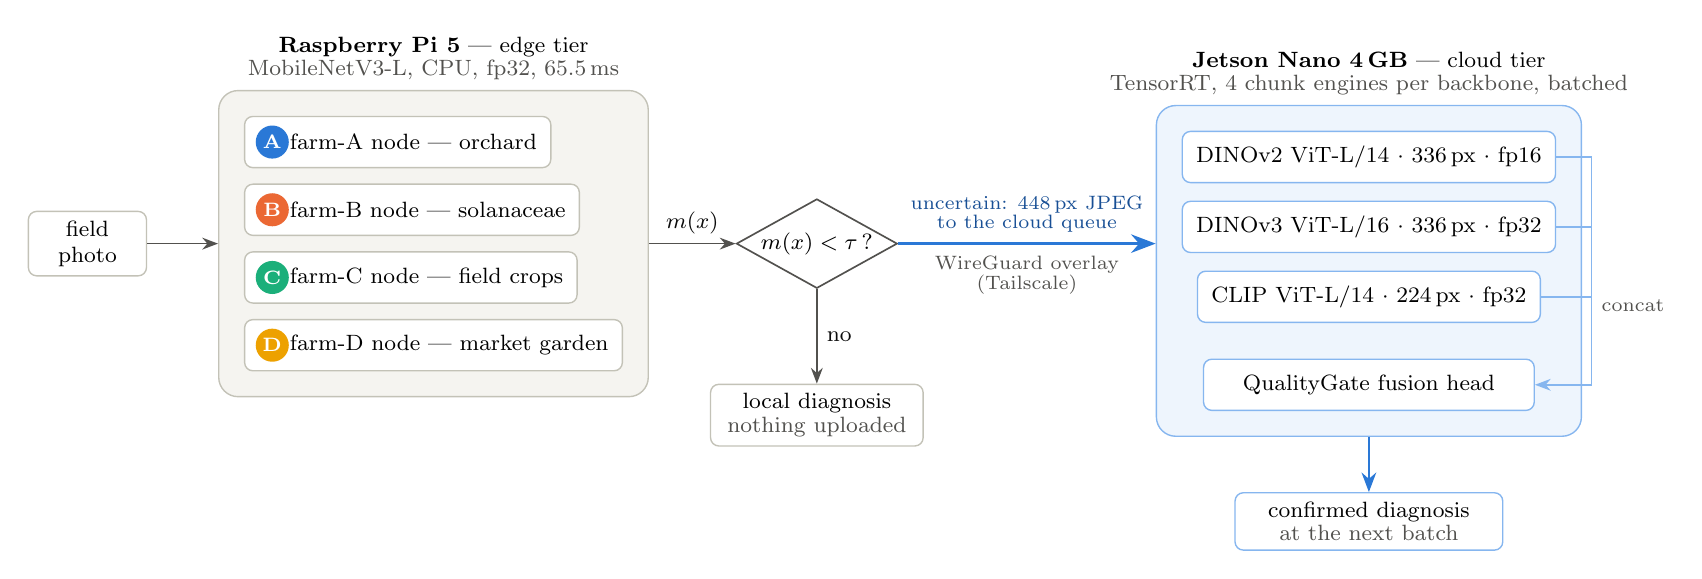
\begin{tikzpicture}[
  font=\footnotesize, >=Stealth, node distance=2.2mm and 9mm,
  proc/.style={draw=#1, rounded corners=3pt, align=center, minimum height=6.5mm,
               fill=white, line width=0.5pt, inner xsep=5pt},
  proc/.default=axisgray,
  dec/.style={draw=inkgray, diamond, aspect=1.8, align=center, inner sep=0.6pt,
              fill=white, line width=0.6pt},
  grp/.style={rounded corners=7pt, inner sep=3.2mm, line width=0.5pt},
  farm/.style={circle, fill=#1, text=white, inner sep=0pt, minimum size=4.2mm,
               font=\scriptsize\bfseries}]
  % ---- edge: Raspberry Pi 5 with four farm nodes
  \foreach \f/\c/\t [count=\i] in {A/farmA/orchard, B/farmB/solanaceae, C/farmC/field crops, D/farmD/market garden} {
    \node[proc, minimum width=34mm, anchor=west] (f\f) at (0, -\i*8.6mm) {\hspace{4mm}farm-\f\ node --- \t};
    \node[farm=\c] at ([xshift=3.6mm]f\f.west) {\f};
  }
  \begin{scope}[on background layer]
    \node[grp, fill=edgefill, draw=edgeline, fit=(fA)(fD),
          label={[align=center, font=\footnotesize]above:{\textbf{Raspberry Pi 5} --- edge tier\\[-1pt]
          {\color{inkgray}MobileNetV3-L, CPU, fp32, 65.5\,ms}}}] (pi) {};
  \end{scope}
  \node[proc, left=9mm of pi, minimum width=15mm] (cam) {field\\photo};
  % ---- decision
  \node[dec, right=11mm of pi] (d) {$m(x)<\tau$\,?};
  \node[proc, below=12mm of d, minimum width=27mm] (loc) {local diagnosis\\[-1pt]{\color{inkgray}nothing uploaded}};
  % ---- cloud: Jetson Nano 4 GB
  \node[proc=cloudline, right=36mm of d, yshift=11mm, minimum width=42mm] (b1)
        {DINOv2 ViT-L/14 $\cdot$ 336\,px $\cdot$ fp16};
  \node[proc=cloudline, below=of b1, minimum width=42mm] (b2) {DINOv3 ViT-L/16 $\cdot$ 336\,px $\cdot$ fp32};
  \node[proc=cloudline, below=of b2, minimum width=42mm] (b3) {CLIP ViT-L/14 $\cdot$ 224\,px $\cdot$ fp32};
  \node[proc=cloudline, below=4.5mm of b3, minimum width=42mm] (qg) {QualityGate fusion head};
  \begin{scope}[on background layer]
    \node[grp, fill=cloudfill, draw=cloudline, fit=(b1)(qg),
          label={[align=center, font=\footnotesize]above:{\textbf{Jetson Nano 4\,GB} --- cloud tier\\[-1pt]
          {\color{inkgray}TensorRT, 4 chunk engines per backbone, batched}}}] (jn) {};
  \end{scope}
  \node[proc=cloudline, below=7mm of jn, minimum width=34mm] (cl) {confirmed diagnosis\\[-1pt]{\color{inkgray}at the next batch}};
  % ---- arrows
  \draw[->, inkgray, line width=0.6pt] (cam) -- (pi);
  \draw[->, inkgray, line width=0.6pt] (pi) -- node[above, text=ink]{$m(x)$} (d);
  \draw[->, inkgray, line width=0.6pt] (d) -- node[right, text=ink]{no} (loc);
  \draw[->, accent, line width=1.3pt] (d) -- node[above, text=accentdark, align=center, font=\scriptsize]
        {uncertain: 448\,px JPEG\\[-1pt]to the cloud queue} (d -| jn.west);
  \node[below=0.4mm of $(d.east)!0.5!(d -| jn.west)$, font=\scriptsize, text=inkgray, align=center]
        {WireGuard overlay\\[-1pt](Tailscale)};
  \coordinate (mg) at ($(b2.east)+(4.5mm,0)$);
  \draw[cloudline, line width=0.6pt] (b1.east) -| (mg);
  \draw[cloudline, line width=0.6pt] (b3.east) -| (mg);
  \draw[cloudline, line width=0.6pt] (b2.east) -- (mg);
  \draw[->, cloudline, line width=0.6pt] (mg) |- node[pos=0.25, right, text=inkgray, font=\scriptsize]{concat} (qg.east);
  \draw[->, accent, line width=0.9pt] (jn) -- (cl);
\end{tikzpicture}}
\caption{System overview: selective edge--cloud escalation.}
\label{fig:system}
\end{figure*}

\subsection{System architecture}
\label{sec:architecture}
Figure~\ref{fig:system} summarises how one image travels through the system: each farm node runs the edge model on every image, answers the farmer without waiting for the ensemble and computes the margin $m(x)$ between its two most probable classes; only uncertain images ($m<\tau$) are uploaded, resized to a 448\,px shorter side, to the cloud node's queue, which is processed in batches, backbone by backbone with one chunk engine in memory at a time (Section~\ref{sec:batch}), and the ensemble's diagnosis is returned. All traffic travels over an encrypted WireGuard overlay. Figure~\ref{fig:architecture} shows the system as deployed. It has three
tiers, each a set of independent services that communicate only through
small HTTP/JSON interfaces. The \emph{edge tier} runs one service per farm
(\texttt{plant-edge-farm@A}\ldots\texttt{D}, managed by systemd on the
Raspberry Pi~5); the \emph{cloud tier} runs a single service
(\texttt{plant-cloud-trt} on the Jetson Nano); and an \emph{operations
tier} on a workstation drives the experiment, records every event and
displays the fleet's state. Four paths connect them. A capture is sent to
its farm's edge service (path~1), which answers with its own diagnosis,
margin and upload size (path~2). Only if the margin is below $\tau$ does
the edge service also resize the image and place it on the cloud's queue
(path~3), before answering; the answer therefore waits for the upload to
be acknowledged but never for the cloud's diagnosis. Twice
a day the queue is processed as one batch and the ensemble's confirmed
diagnoses are returned (path~4). Because the tiers share nothing but these
interfaces, a farm can be added by starting one more edge service, and the
cloud tier can move from the Nano to any larger machine without changing
the edge.

\begin{figure*}[!htbp]
\centering
\resizebox{\linewidth}{!}{%
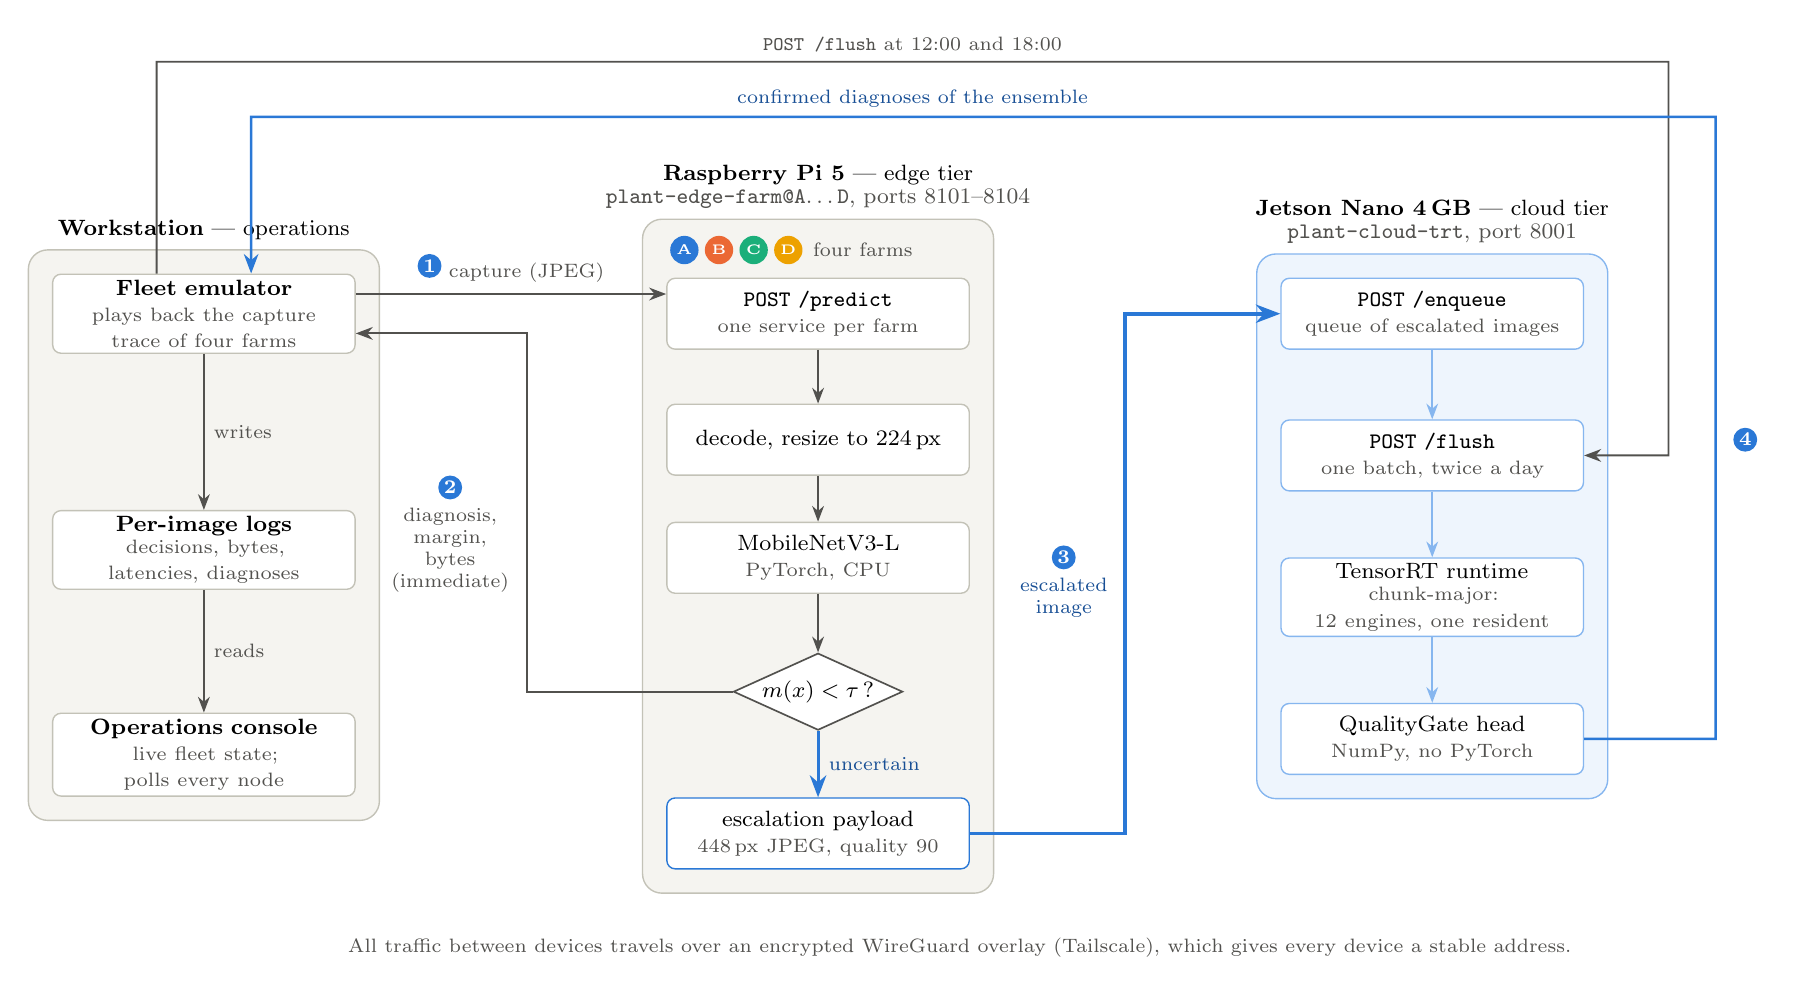
\begin{tikzpicture}[
  font=\footnotesize, >=Stealth,
  box/.style={draw=#1, rounded corners=3pt, align=center, fill=white, line width=0.5pt,
              text width=37mm, minimum height=9mm, inner sep=2pt},
  box/.default=axisgray,
  dec/.style={draw=inkgray, diamond, aspect=2.2, align=center, inner sep=0.5pt, fill=white,
              line width=0.6pt},
  grp/.style={rounded corners=7pt, inner sep=3mm, line width=0.5pt},
  num/.style={circle, fill=accent, text=white, inner sep=0.8pt, font=\scriptsize\bfseries},
  lab/.style={font=\scriptsize, text=inkgray, align=center}]
  % ---- operations tier (workstation)
  \node[box] (sim)  at (22mm,-14mm) {\textbf{Fleet emulator}\\{\color{inkgray}\scriptsize plays back the capture trace of four farms}};
  \node[box] (logs) at (22mm,-44mm) {\textbf{Per-image logs}\\{\color{inkgray}\scriptsize decisions, bytes,\\latencies, diagnoses}};
  \node[box] (con)  at (22mm,-70mm) {\textbf{Operations console}\\{\color{inkgray}\scriptsize live fleet state; polls every node}};
  \begin{scope}[on background layer]
    \node[grp, fill=edgefill, draw=edgeline, fit=(sim)(logs)(con),
          label={[align=center, font=\footnotesize]above:{\textbf{Workstation} --- operations}}] {};
  \end{scope}
  % ---- edge tier (Raspberry Pi 5)
  \node[box] (p1) at (100mm,-14mm) {\texttt{POST /predict}\\{\color{inkgray}\scriptsize one service per farm}};
  \node[box] (p2) at (100mm,-30mm) {decode, resize to 224\,px};
  \node[box] (p3) at (100mm,-45mm) {MobileNetV3-L\\{\color{inkgray}\scriptsize PyTorch, CPU}};
  \node[dec] (p4) at (100mm,-62mm) {$m(x)<\tau$\,?};
  \node[box=accent] (p5) at (100mm,-80mm) {escalation payload\\{\color{inkgray}\scriptsize 448\,px JPEG, quality 90}};
  \coordinate (ptop) at (100mm,-5mm);
  \begin{scope}[on background layer]
    \node[grp, fill=edgefill, draw=edgeline, fit=(ptop)(p1)(p5),
          label={[align=center, font=\footnotesize]above:{\textbf{Raspberry Pi 5} --- edge tier\\[-1pt]
          {\color{inkgray}\texttt{plant-edge-farm@A}\ldots\texttt{D}, ports 8101--8104}}}] (pi) {};
  \end{scope}
  \foreach \f/\c [count=\i] in {A/farmA, B/farmB, C/farmC, D/farmD}
    \node[circle, fill=\c, text=white, inner sep=0pt, minimum size=3.6mm, font=\tiny\bfseries]
      at ($(pi.north west)+(1mm+\i*4.4mm,-4mm)$) {\f};
  \node[lab, anchor=west] at ($(pi.north west)+(20.5mm,-4mm)$) {four farms};
  % ---- cloud tier (Jetson Nano)
  \node[box=cloudline] (n1) at (178mm,-14mm) {\texttt{POST /enqueue}\\{\color{inkgray}\scriptsize queue of escalated images}};
  \node[box=cloudline] (n2) at (178mm,-32mm) {\texttt{POST /flush}\\{\color{inkgray}\scriptsize one batch, twice a day}};
  \node[box=cloudline] (n3) at (178mm,-50mm) {TensorRT runtime\\{\color{inkgray}\scriptsize chunk-major:\\12 engines, one resident}};
  \node[box=cloudline] (n4) at (178mm,-68mm) {QualityGate head\\{\color{inkgray}\scriptsize NumPy, no PyTorch}};
  \begin{scope}[on background layer]
    \node[grp, fill=cloudfill, draw=cloudline, fit=(n1)(n4),
          label={[align=center, font=\footnotesize]above:{\textbf{Jetson Nano 4\,GB} --- cloud tier\\[-1pt]
          {\color{inkgray}\texttt{plant-cloud-trt}, port 8001}}}] (jn) {};
  \end{scope}
  % ---- edge internals
  \foreach \a/\b in {p1/p2, p2/p3, p3/p4} \draw[->, inkgray, line width=0.6pt] (\a) -- (\b);
  \draw[->, accent, line width=1.1pt] (p4) -- node[right, lab, text=accentdark]{uncertain} (p5);
  % ---- cloud internals
  \foreach \a/\b in {n1/n2, n2/n3, n3/n4} \draw[->, cloudline, line width=0.6pt] (\a) -- (\b);
  % ---- path 1: capture
  \draw[->, inkgray, line width=0.7pt] ([yshift=2.5mm]sim.east) -- ([yshift=2.5mm]sim.east -| p1.west);
  \node[lab, anchor=south] at ([yshift=2.7mm]$(sim.east)!0.5!(sim.east -| p1.west)$) {\tikz\node[num]{1}; capture (JPEG)};
  % ---- path 2: immediate answer
  \draw[->, inkgray, line width=0.7pt] (p4.west) -- (63mm,-62mm) |- ([yshift=-2.5mm]sim.east);
  \node[lab, anchor=east] at (62mm,-42mm) {\tikz\node[num]{2};\\diagnosis,\\margin,\\bytes\\(immediate)};
  % ---- path 3: escalation
  \draw[->, accent, line width=1.3pt] (p5.east) -- (139mm,-80mm) |- (n1.west);
  \node[lab, anchor=east, text=accentdark] at (138mm,-48mm) {\tikz\node[num]{3};\\escalated\\image};
  % ---- path 4: batch trigger and confirmed diagnoses
  \draw[->, inkgray, line width=0.7pt] ([xshift=-6mm]sim.north) -- (16mm,18mm) -- (208mm,18mm) -- (208mm,-32mm) -- (n2.east);
  \node[lab, anchor=south] at (112mm,18mm) {\texttt{POST /flush} at 12:00 and 18:00};
  \draw[->, accent, line width=0.9pt] (n4.east) -- (214mm,-68mm) -- (214mm,11mm) -- (28mm,11mm) -- ([xshift=6mm]sim.north);
  \node[lab, anchor=south, text=accentdark] at (112mm,11mm) {confirmed diagnoses of the ensemble};
  \node[lab, anchor=west] at (215mm,-30mm) {\tikz\node[num]{4};};
  % ---- logging and monitoring
  \draw[->, inkgray, line width=0.6pt] (sim) -- node[right, lab]{writes} (logs);
  \draw[->, inkgray, line width=0.6pt] (logs) -- node[right, lab]{reads} (con);
  % ---- overlay
  \node[lab, anchor=north] at (118mm,-92mm) {All traffic between devices travels over an encrypted WireGuard overlay (Tailscale), which gives every device a stable address.};
\end{tikzpicture}}
\caption{System architecture as deployed.}
\label{fig:architecture}
\end{figure*}

\subsection{Hardware and software}
Table~\ref{tab:hardware} summarises the
testbed\IfFileExists{figures/setup_photo.jpg}{, photographed in
Fig.~\ref{fig:setup} (\mbox{\ref{app:testbed}})}{}. The edge is a
Raspberry Pi~5 running the edge model in PyTorch on its CPU. The cloud
node is a 4\,GB Jetson Nano, a low-cost embedded GPU module, chosen
deliberately: if a three-backbone foundation ensemble can be served from
a device of this class, the ``cloud'' in our architecture can be a
cooperative- or farm-level box rather than a data centre. The nodes
communicate over a WireGuard-based overlay network
\citep{donenfeld2017wireguard} (Tailscale), which encrypts all traffic
and gives each device a stable address regardless of its physical
network. Both servers expose a small HTTP/JSON interface in which images
travel as base64-encoded JPEG. All byte counts in this paper are those of
the JPEG payload; the base64 text encoding of our prototype adds a third
on top of them, an overhead that a binary upload removes and that leaves
every reduction factor unchanged.

\begin{table}[!htbp]
\centering
\caption{Embedded testbed.}
\label{tab:hardware}
\small
\begin{tabular}{@{}L{0.15\linewidth}L{0.36\linewidth}L{0.42\linewidth}@{}}
\toprule
 & \textbf{Edge} & \textbf{Cloud} \\
\midrule
Device        & Raspberry Pi 5 Model B & Jetson Nano Developer Kit \\
Processor     & 4$\times$ Cortex-A76, 2.4\,GHz & 4$\times$ Cortex-A57 + 128-core Maxwell GPU \\
Memory        & 16\,GB & 4\,GB (shared CPU/GPU) \\
OS            & Debian 13 & Ubuntu 18.04 (JetPack 4.6.1, L4T R32.7.1) \\
Runtime       & Python 3.13, PyTorch 2.6 (CPU) & Python 3.6, TensorRT 8.2.1, CUDA 10.2 \\
Model         & MobileNetV3-L, fp32 & DINOv2-L (fp16), DINOv3-L and CLIP-L (fp32); 4 chunk engines each \\
Power mode    & default (\texttt{ondemand}) & MAXN \\
\bottomrule
\end{tabular}
\end{table}

\subsection{Edge node}
\label{sec:edge-node}
Each edge node is a stateless HTTP service. For every image it decodes
the JPEG, applies the edge model, computes the margin and, if
$m(x)<\tau$, forwards the image to the cloud node; the uploaded byte count
is recorded per image once the cloud acknowledges it. Escalation is
\emph{deferred}: the node uploads the image to the cloud node's queue and
returns its own label as soon as the upload is acknowledged, so the
farmer never waits for the ensemble's diagnosis, which follows when the
queue is processed (Section~\ref{sec:batch}). The upload itself, however,
is on the answer path of our prototype: it adds \RNetMs\,ms (median) on
the testbed's local network, about \RUplinkS\,s for a median payload on a
\RUplinkMbps\,Mbit/s rural uplink, and up to the 60\,s request timeout if
the cloud node cannot be reached, after which the node answers with its
own label. All latencies reported in this paper include this upload. A
production node should upload from a background queue so that the answer
never waits for the network; the released edge server offers this as an
option, which was added after the measurements and is not evaluated
here.

\paragraph{Escalation payload} Field photographs are often far larger than
the cloud model needs: some PlantWild images exceed 12 megapixels, while
the cloud backbones operate at 224--336\,px. Uploading at the camera's
resolution therefore wastes most of the escalated bytes. The edge instead
resizes an escalated image so that its shorter side is 448\,px and encodes
it as JPEG at quality~90. The policy is chosen on the validation split,
so that no test image informs a design choice: Table~\ref{tab:payload}
shows the trade-off on its \RPayN images, measured with the reference
cloud pipeline. Agreement is the fraction of images for which the cloud's
diagnosis from the payload equals its diagnosis from the original file,
and KB are mean sizes over the same images (the original files average
\RPayOrigKb\,KB on disk). Among the downscaled payloads, 448\,px at
quality~90 keeps the highest agreement (\RPayFourFourEightAgree) with no
loss of cloud accuracy, for \RPayRatio$\times$ fewer bytes than the
full-resolution image at the same quality; a 336\,px payload would save
another 30\,\% of the bytes at a small cost in agreement and accuracy.
The always-cloud
baseline in the deployment uses the identical payload, so the measured
reduction factor isolates the effect of selective escalation.

\begin{table}[!htbp]
\centering
\caption{Escalation payload policy (validation split).}
\label{tab:payload}
\small
\begin{tabular}{@{}lrrr@{}}
\toprule
\textbf{Payload} & \textbf{KB / escalation} & \textbf{Agreement} & \textbf{Cloud top-1} \\
\midrule
Original file                     & \RPayOrigKb & --- & \RPayOrigAcc \\
Full resolution, JPEG q90         & \RPayFullKb & \RPayFullAgree & \RPayFullAcc \\
\textbf{Shorter side 448\,px, q90} & \textbf{\RPayFourFourEightKb} & \textbf{\RPayFourFourEightAgree} & \textbf{\RPayFourFourEightAcc} \\
Shorter side 336\,px, q95         & \RPayThreeThreeSixQNinetyFiveKb & \RPayThreeThreeSixQNinetyFiveAgree & \RPayThreeThreeSixQNinetyFiveAcc \\
Shorter side 336\,px, q90         & \RPayThreeThreeSixKb & \RPayThreeThreeSixAgree & \RPayThreeThreeSixAcc \\
Shorter side 224\,px, q90         & \RPayTwoTwoFourKb & \RPayTwoTwoFourAgree & \RPayTwoTwoFourAcc \\
\bottomrule
\end{tabular}
\end{table} If the
cloud is unreachable, the node falls back to its own prediction and
records the failure, so that an outage degrades accuracy rather than
availability. The deployment uses the validation-calibrated $\tau = 0.138$
(Section~\ref{sec:router}).

\subsection{Trace-driven emulation of a multi-farm week}
\label{sec:fleet}
A field deployment spans days, with hours between captures. To study
that regime within an experimental session we use trace-driven,
hardware-in-the-loop emulation rather than simulation: a recorded
workload (the test images, arranged into a week of captures) is played back through the real devices and the real network, so that every inference,
every transfer and every byte is executed and measured rather than
modelled. Only the clock is compressed --- idle time between captures is
skipped --- and we refer to its time axis as simulated hours and days. We
call this experiment an \emph{emulated deployment}, or the
\emph{emulation} for short. It was run twice: the \emph{baseline
deployment} uses the original edge model, and the \emph{distilled
deployment} (Section~\ref{sec:res-improved}) the edge model distilled
from the ensemble.

\paragraph{Virtual farms} Four farm nodes run as independent edge
processes on the Raspberry Pi~5, each with its own identifier, port,
routing decisions and connection to the cloud node; the cloud therefore
serves four distinct clients. Farms differ in what they grow: the 89
classes are grouped by crop into an orchard (apple, banana, blueberry,
cherry, citrus, coffee, grape, maple, peach, plum, raspberry,
strawberry; 1\,360 test images), a solanaceous-crop farm (bell pepper,
eggplant, potato, tobacco, tomato; 701), a field-crop farm (bean, corn,
garlic, ginger, rice, soybean; 707) and a market garden (basil,
broccoli, cabbage, carrot, cauliflower, celery, cucumber, lettuce,
squash, zucchini; 909). Together they cover the full 3\,677-image test
split exactly once.

\paragraph{Schedule} Each farm's images are spread evenly over the
daylight hours (07:00--19:00) of seven simulated days, giving 84 capture
hours per farm; within an hour, requests from different farms are
interleaved. One simulated hour lasts at least one second of wall-clock
time and is stretched when its captures take longer, so the emulation never drops or overlaps work.

\paragraph{What is and is not emulated} Requests are issued one at a
time, so every edge latency is that of a single request on an otherwise
idle device --- exactly what a farm owning its own Pi would observe.
Upload sizes, escalation decisions, diagnoses and per-stage latencies
(edge inference, network, cloud inference) are measured for every image.
What the emulation compresses is idle time; what it emulates is the
multiplicity of edge devices. Table~\ref{tab:provenance} lists the
provenance of every quantity reported in this paper.

\begin{table}[!htbp]
\centering
\caption{Provenance of the reported quantities.}
\label{tab:provenance}
\small
\begin{tabular}{@{}L{0.42\linewidth}L{0.52\linewidth}@{}}
\toprule
\textbf{Quantity} & \textbf{Provenance} \\
\midrule
Accuracy, escalation rate (offline) & measured on the PlantWild test split \\
Bandwidth reduction factor $1/r$     & measured (independent of image size) \\
Absolute KB per image (offline)     & escalation rate $\times$ measured mean payload $S$ \\
Absolute KB per image (deployment)  & measured JPEG bytes of every upload \\
Edge latency                        & measured on the Raspberry Pi~5 \\
Cloud latency                       & measured on the Jetson Nano \\
Cloud memory and energy             & measured on the Jetson Nano (\texttt{tegrastats}: RAM, board input power) \\
Edge energy                         & measured on the Raspberry Pi~5 (power-management IC: SoC and memory rails, a lower bound) \\
Distillation and loop pilot         & offline, on the workstation; test split as in Section~\ref{sec:data} \\
Network latency                     & measured over the overlay; local network, i.e.\ a best case for rural links \\
Four farms                          & four processes on one physical Pi (emulated multiplicity) \\
Seven days                          & simulated clock; idle time compressed, work not compressed \\
\bottomrule
\end{tabular}
\end{table}

% =====================================================================
\section{Running a foundation-model ensemble on end-of-life embedded hardware}
\label{sec:port}
% =====================================================================

The Jetson Nano is typical of hardware that farms, cooperatives and
agricultural schools already own or can buy cheaply, but that the
software ecosystem has left behind. NVIDIA's last software release for it
(JetPack~4.6) ships Ubuntu~18.04, Python~3.6, CUDA~10.2 and TensorRT~8.2,
whereas the reference cloud implementation relies on PyTorch~2,
\texttt{timm} and \texttt{open\_clip}, none of which runs on that stack;
DINOv3 in particular requires a far newer toolchain. Memory is the second
wall: the board's 4\,GB are shared by CPU and GPU, while the fp32 weights
of the three backbones alone occupy about 3.4\,GB. Rather than rebuild a
framework stack on the device, we treated the port as an engineering
problem and solved it with five principles, each of which transfers to
other legacy accelerators. Table~\ref{tab:port} summarises the decisive
obstacles; \mbox{\ref{app:adaptations}} lists all of the adaptations the
port required.

\begin{figure*}[!htbp]
\centering
\resizebox{\linewidth}{!}{%
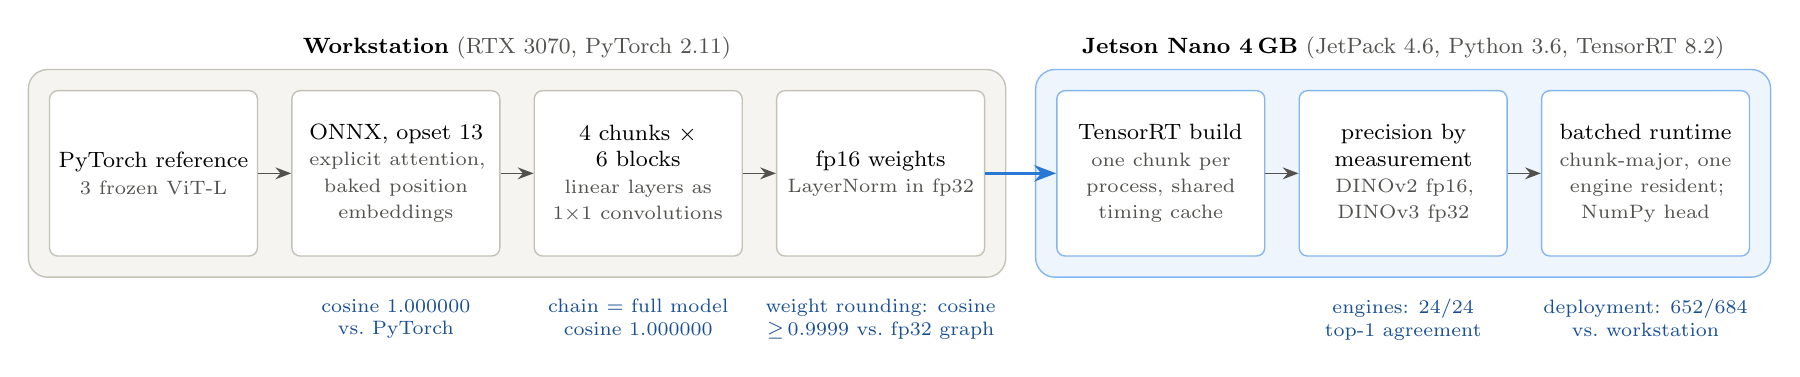
\begin{tikzpicture}[
  font=\footnotesize, >=Stealth, node distance=3mm and 4.2mm,
  st/.style={draw=#1, rounded corners=3pt, align=center, fill=white, line width=0.5pt,
             minimum height=21mm, text width=25mm, inner sep=2pt},
  st/.default=axisgray,
  chk/.style={font=\scriptsize, text=accentdark, align=center},
  grp/.style={rounded corners=7pt, inner sep=2.6mm, line width=0.5pt}]
  % ---- workstation
  \node[st] (w1) {PyTorch reference\\{\color{inkgray}\scriptsize 3 frozen ViT-L}};
  \node[st, right=of w1] (w2) {ONNX, opset 13\\{\color{inkgray}\scriptsize explicit attention, baked position embeddings}};
  \node[st, right=of w2] (w3) {4 chunks $\times$ 6 blocks\\{\color{inkgray}\scriptsize linear layers as 1$\times$1 convolutions}};
  \node[st, right=of w3] (w4) {fp16 weights\\{\color{inkgray}\scriptsize LayerNorm in fp32}};
  \begin{scope}[on background layer]
    \node[grp, fill=edgefill, draw=edgeline, fit=(w1)(w2)(w3)(w4),
          label={[font=\footnotesize]above:{\textbf{Workstation} {\color{inkgray}(RTX~3070, PyTorch~2.11)}}}] (ws) {};
  \end{scope}
  % ---- Nano
  \node[st=cloudline, right=9mm of w4] (n1) {TensorRT build\\{\color{inkgray}\scriptsize one chunk per process, shared timing cache}};
  \node[st=cloudline, right=of n1] (n2) {precision by measurement\\{\color{inkgray}\scriptsize DINOv2 fp16, DINOv3 fp32}};
  \node[st=cloudline, right=of n2] (n3) {batched runtime\\{\color{inkgray}\scriptsize chunk-major, one engine resident; NumPy head}};
  \begin{scope}[on background layer]
    \node[grp, fill=cloudfill, draw=cloudline, fit=(n1)(n2)(n3),
          label={[font=\footnotesize]above:{\textbf{Jetson Nano 4\,GB} {\color{inkgray}(JetPack~4.6, Python~3.6, TensorRT~8.2)}}}] (nano) {};
  \end{scope}
  \foreach \a/\b in {w1/w2, w2/w3, w3/w4, n1/n2, n2/n3} \draw[->, inkgray, line width=0.6pt] (\a) -- (\b);
  \draw[->, accent, line width=1.1pt] (w4) -- (n1);
  % ---- checks
  \foreach \n/\t in {w2/{cosine 1.000000\\vs.\ PyTorch}, w3/{chain = full model\\cosine 1.000000},
                     w4/{weight rounding: cosine\\$\geq$\,0.9999 vs.\ fp32 graph}, n2/{engines: \REngAgree\\top-1 agreement},
                     n3/{deployment: \RCloudAgreeFleet\\vs.\ workstation}}
    \node[chk, anchor=north] at ([yshift=-1.5mm]\n |- nano.south) {\t};
\end{tikzpicture}}
\caption{Porting the cloud ensemble to the Jetson Nano.}
\label{fig:port-pipeline}
\end{figure*}

\begin{table*}[!htbp]
\centering
\caption{Decisive obstacles of the port, their causes and the adaptations that resolved them.}
\label{tab:port}
\footnotesize
\begin{tabular}{@{}L{0.19\linewidth}L{0.23\linewidth}L{0.28\linewidth}L{0.20\linewidth}@{}}
\toprule
\textbf{Obstacle} & \textbf{Cause} & \textbf{Adaptation} & \textbf{Evidence} \\
\midrule
Reference server cannot run & JetPack~4: Python~3.6, CUDA~10.2 & ONNX export on the workstation; torch-free NumPy server & graphs cosine 1.000000; preprocessing bit-identical \\
Operators rejected by TensorRT~8.2 & fused attention, cubic resize, shape-dependent position embeddings & explicit attention; position embeddings baked as constants; constant folding & no unsupported operator left \\
A whole ViT-L cannot be compiled & ONNX parser alone peaks at 2.75\,GB & fp16 weights; four chunks of six blocks & chained chunks cosine 1.000000 \\
969\,MB of device memory per chunk & weights fused into one opaque kernel graph & every linear layer as a $1{\times}1$ convolution & engine 612\,$\rightarrow$\,157\,MB \\
NaN features from DINOv3 & residual stream $1.6{\times}10^{5}$, above the fp16 range & precision chosen per backbone from measured ranges & DINOv3 engine cosine \REngCosMinDinoThree \\
Only 9 of 12 chunks fit & ${\approx}$0.35\,GB per loaded fp16 chunk; fp32 chunks twice as large & chunk-major batched inference, deferred escalation & peak \RNanoPeakGB\,GB of \RNanoTotalGB\,GB \\
Residual on-device deviation & Pillow~8.4 links a different JPEG decoder & isolated (decoding, not resampling) and measured; accepted with stock JetPack~4 packages & \RCloudAgreeFleet\ agreement in deployment \\
\bottomrule
\end{tabular}
\end{table*}

\subsection{Decouple the model from its framework}
On the workstation, each backbone is exported to ONNX \citep{onnx2019} at
opset~13, the newest opset that TensorRT~8.2 parses
(Fig.~\ref{fig:port-pipeline}). The blue labels in the figure give the fidelity check passed at each stage, detailed in Section~\ref{sec:verify}. Fused scaled-dot-product attention has no
opset-13 equivalent, so attention is traced in its explicit
$\mathrm{softmax}(QK^\top/\sqrt{d})V$ form, which is mathematically
identical. Operations that depend on the input shape --- DINOv2's bicubic
resizing of its position grid, DINOv3's rotary position embedding --- are
evaluated once for the fixed input size and stored as constants, and an
export is rejected if any operator unsupported by TensorRT~8.2 remains.
Image preprocessing is re-implemented without PyTorch --- Pillow
decodes the JPEG and performs the bicubic resize, as torchvision does,
and NumPy crops, normalises and lays out the tensor --- and the
QualityGate head of Eq.~\eqref{eq:qg} is re-implemented in NumPy, so the
serving process on the Nano needs neither PyTorch nor its dependencies.

\subsection{Compile within the memory ceiling}
A whole ViT-L cannot be compiled on the Nano: TensorRT's ONNX parser alone
peaks at 2.75\,GB of RAM for a 0.6\,GB fp16 graph, before the builder has
started (Fig.~\ref{fig:port}b). Figure~\ref{fig:port}b compares the memory each step of the port needs with the board's shared CPU/GPU memory; the grey bars are the steps that did not fit. Each backbone is therefore exported as
four consecutive chunks of six transformer blocks (the first also holding
the patch embedding, the last the pooling and projection), converted to
fp16 weights with LayerNorm arithmetic kept in fp32, and compiled into a
TensorRT engine \citep{nvidia2022tensorrt} one chunk at a time. Weights
are stored in fp16 for all three backbones; the precision in which an
engine \emph{computes} is chosen per backbone when it is built (next
subsection); at run time
the chunks are chained and compute exactly the full forward pass (cosine
1.000000 against the unsplit model). A second, less visible limit
followed: TensorRT~8.2 fuses transformer layers whose weights enter
through matrix products into one opaque kernel graph, which held 969\,MB of
device memory for six blocks --- about 13\,bytes per parameter. Expressing
every linear layer as the equivalent $1{\times}1$ convolution keeps the
weights in TensorRT's native layers and shrinks the engine for the same six
blocks from 612 to 157\,MB. The residual stream keeps its (batch, tokens,
channels) layout: each linear layer reshapes its input to a
$1 \times C \times (B\,N) \times 1$ tensor, applies the convolution and
reshapes the result back, and attention is computed on (batch, heads,
tokens, head dimension) tensors as before.

\begin{figure*}[!htbp]
\centering
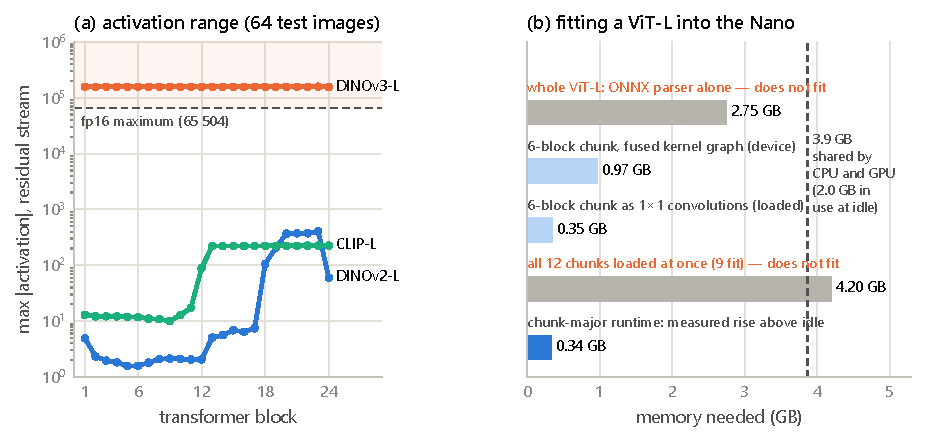
\includegraphics[width=\linewidth]{figures/fig_port.pdf}
\caption{Activation ranges and memory requirements of the port. (a)~Largest residual-stream activation per transformer block. (b)~Memory needed at each step of the port.}
\label{fig:port}
\end{figure*}

\subsection{Choose precision by measurement}
Half precision halves weights and load time, but it does not suit every
backbone. Our first fp16 build of DINOv3 produced NaN features. The
natural suspect, LayerNorm overflowing in fp16, was wrong: pinning
LayerNorm, and then every non-convolution layer, to fp32 changed nothing.
Profiling the reference model (Fig.~\ref{fig:port}a) on \RActNImg test images located the cause:
DINOv3's residual stream carries activations of up to \RActDinoThree from
its first block onwards, beyond the largest fp16 value (65\,504), whereas
DINOv2 and CLIP peak at \RActDinoTwo and \RActClip. DINOv2 therefore runs
in fp16 and DINOv3 in fp32. Our workstation check of the fp16-weight
graphs (Table~\ref{tab:fidelity}) could not have revealed the overflow:
onnxruntime's CPU provider has no fp16 kernels for these operators and
computes them in fp32, so the check validated the rounding of the
weights, not fp16 arithmetic --- run there, the first DINOv3 chunk's
hidden state reaches $1.57{\times}10^{5}$ without overflowing. An fp32
engine is built from the same fp16-weight graph with every layer pinned
to fp32 by TensorRT's precision constraints: it keeps the rounded weights
but computes in fp32, and the rounding is harmless, as the engines
reproduce the fp32 reference to a cosine of at least
\REngCosMinDinoThree. CLIP was moved to fp32 as well while we
investigated a deviation that we later traced to the image library rather
than to precision (Section~\ref{sec:verify}). A later check confirmed
that fp32 is unnecessary for CLIP: fp16 CLIP engines reproduce the fp32
ones to a cosine of at least \RClipSixteenCos on the 24 reference images,
with the same pipeline agreement, while cutting CLIP's compute from
\RClipThirtyTwoMs to \RClipSixteenMs\,ms per image and its loading from
\RClipThirtyTwoLoadS to \RClipSixteenLoadS\,s. The baseline deployment used fp32 CLIP; fp16 is the better choice for new deployments.

\subsection{Run within the memory ceiling: chunk-major batched inference}
\label{sec:batch}
Even in compact form, a loaded fp16 chunk engine occupies about 0.35\,GB of
the Nano's shared memory (157\,MB of weights on the device plus the
runtime's host-side copy and scratch), and we measured, with fp16 engines
for all three backbones, that at most nine of the twelve chunks can be
resident at once, even with a single activation buffer shared by all of
them. The deployed mix is larger still: an fp32 chunk engine occupies
\RTrtChunkThirtyTwoMB\,MB on disk against \RTrtChunkSixteenMB\,MB for an
fp16 one, and the twelve deployed engines total \RTrtDiskGB\,GB. The full ensemble therefore cannot answer
requests synchronously on this device. We resolve the conflict with a
design that matches how diagnoses are used on farms: an escalated image is
\emph{queued} on the cloud node, and the edge returns its own label to the
farmer as soon as the image is queued. The cloud node processes its queue in batches,
chunk by chunk: it loads the first chunk of DINOv2, passes every queued
image through it, frees it, loads the next chunk, and so on through
DINOv3 and CLIP, keeping each image's intermediate hidden state (up to
2.4\,MB for DINOv2's 577 tokens) in host memory, and finally applies the head. With its decoded
payload and preprocessed input, a queued image holds about 4.5\,MB during a
batch, so the released server processes queues of more than 128 images in
sub-batches of 128 (about 0.6\,GB), reloading the engines for each; this
cap was added after the measurements, in which no batch exceeded 61
images. At no time is more
than one chunk engine resident. In the emulation the queue is processed twice
a day, after the 12:00 and 18:00 captures, so every escalated image
receives the ensemble's diagnosis on the day it was taken; the batch
interval trades confirmation delay for model-loading overhead. The server
also implements a synchronous mode with all engines resident, intended for
cloud nodes with more memory; we did not test it.

To quantify the design on the device, we processed \RNanoRuns batches of
\RNanoBatchN escalated images --- the median batch of the baseline deployment, with the
same payload --- while sampling RAM and the board's input power rail with
\texttt{tegrastats} about eight times per second (Fig.~\ref{fig:nano-flush}). In the figure, shading marks the backbone being processed; the twelve dips in power are the twelve chunk-engine loads, between which the GPU passes all queued images through the resident chunk. The dashed lines mark the board's total shared memory and its idle power draw.
Memory use never exceeds \RNanoPeakGB\,GB of the \RNanoTotalGB\,GB
(\RNanoIdleGB\,GB at idle, including the operating system and the idle
server): processing a batch adds about \RNanoRiseGB\,GB on average, the
footprint of one chunk engine --- up to \RNanoRiseThirtyTwoGB\,GB while an
fp32 engine (DINOv3, CLIP) is resident and \RNanoRiseSixteenGB\,GB for
the fp16 DINOv2. The board draws \RNanoMeanW\,W on average while processing a batch
(\RNanoIdleW\,W at idle, \RNanoMaxW\,W at most), and a batch takes
\RNanoFlushMin\,min. Each escalated image costs \RNanoEImgJ\,J of board
energy including its share of model loading, or \RNanoEIncrImgJ\,J above
the idle draw --- about \RNanoWhPerThousand\,Wh per thousand escalated
images.

\begin{figure*}[!htbp]
\centering
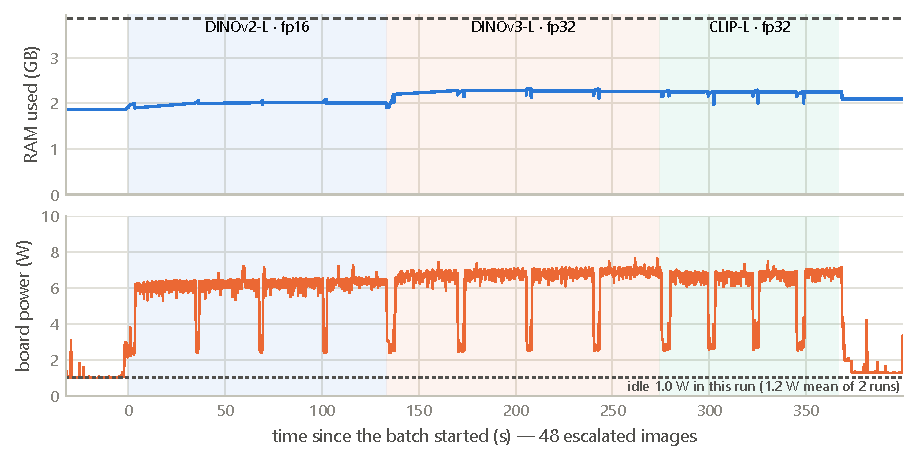
\includegraphics[width=\linewidth]{figures/fig_nano_flush.pdf}
\caption{Jetson Nano memory and board power during one batch of \RNanoBatchN escalated images.}
\label{fig:nano-flush}
\end{figure*}

\subsection{Verify every stage}
\label{sec:verify}
A port is only useful if it computes the same function, so we verify each
stage against the reference pipeline (Table~\ref{tab:fidelity}). Workstation checks compare against the PyTorch reference; checks on the Nano compare TensorRT outputs with reference features computed on the workstation. The
exported graphs match PyTorch to a cosine similarity of 1.000000, the
NumPy preprocessing reproduces the reference tensors exactly, and the
NumPy head matches the original to within $3{\times}10^{-6}$ in the
logits. The reassembled pipeline agrees with the offline reference cloud
predictions on 299 of 300 test images (99.7\,\%). On the Nano, fed the
workstation's preprocessed tensors, the TensorRT engines reproduce the
reference features to a cosine of \REngCosMinDinoThree (DINOv3, fp32),
\REngCosMinClip (CLIP, fp32) and \REngCosMinDinoTwo (DINOv2, fp16) and the
reference top-1 prediction on \REngAgree images. The complete on-device
pipeline agrees on \RAgree: the residual deviation (minimum cosine
\RCosMinAll) does not come from TensorRT but from the image library ---
Pillow~8.4, the last release for JetPack~4's Python~3.6, links a
different JPEG decoder (IJG libjpeg~9) from the workstation's Pillow~12
(libjpeg-turbo~3.1). On the 24 reference images the two decoders return
different values for 36\,\% of pixels, by up to 67/255, so the
preprocessed tensors differ by up to 0.59 normalised units; resampling is
not involved, as both versions resize identical decoded pixels
bit-identically. Over the baseline deployment, the Nano's
diagnosis matches the workstation's offline prediction for
\RCloudAgreeFleet escalated images. Isolating causes in this way ---
engines fed identical tensors, then the complete pipeline --- is what
separated a precision problem that had to be corrected (DINOv3) from a
library difference that we accepted: removing it would require a matched
JPEG decoder on both machines, which stock JetPack~4 packages do not
provide.

\begin{table}[!htbp]
\centering
\caption{Fidelity of the embedded cloud pipeline, stage by stage.}
\label{tab:fidelity}
\small
\begin{tabular}{@{}L{0.28\linewidth}L{0.36\linewidth}r@{}}
\toprule
\textbf{Stage} & \textbf{Check} & \textbf{Result} \\
\midrule
ONNX export (3 backbones)       & cosine vs.\ PyTorch, min over images & 1.000000 \\
Chunking + $1{\times}1$-convolution form & chained chunks vs.\ unsplit model, cosine (PyTorch and ONNX) & 1.000000 \\
fp16 weights, fp32 LayerNorm    & cosine vs.\ fp32 graph, min (computed in fp32: tests weight rounding) & $\geq$\,0.9999 \\
Pillow + NumPy preprocessing    & max.\ abs.\ difference vs.\ torchvision & 0 \\
NumPy QualityGate head          & max.\ abs.\ logit difference & $2.9\times10^{-6}$ \\
Full pipeline                   & agreement with offline cloud predictions & 299/300 (99.7\,\%) \\
\midrule
Edge node (Raspberry Pi 5)      & label agreement with offline edge predictions & 300/300 \\
                                & margin, mean / max.\ abs.\ difference & $8{\times}10^{-4}$ / $7.8{\times}10^{-3}$ \\
\midrule
\multicolumn{3}{@{}l}{\emph{Nano engines, workstation-preprocessed inputs}} \\
TensorRT fp16, DINOv2-L         & cosine vs.\ reference, min / mean & \REngCosMinDinoTwo{} / \REngCosMeanDinoTwo \\
TensorRT fp32, DINOv3-L         & cosine vs.\ reference, min / mean & \REngCosMinDinoThree{} / \REngCosMeanDinoThree \\
TensorRT fp32, CLIP-L           & cosine vs.\ reference, min / mean & \REngCosMinClip{} / \REngCosMeanClip \\
Engines + head                  & top-1 agreement with reference & \REngAgree \\
\multicolumn{3}{@{}l}{\emph{Complete on-device pipeline (Nano image library)}} \\
DINOv2-L / DINOv3-L / CLIP-L    & cosine vs.\ reference, min & \RCosMinDinoTwo{} / \RCosMinDinoThree{} / \RCosMinClip \\
Full pipeline (Nano)            & top-1 agreement with reference & \RAgree \\
Full pipeline (Nano, deployment)    & agreement with offline cloud predictions, every escalated image & \RCloudAgreeFleet \\
\bottomrule
\end{tabular}
\end{table}

% =====================================================================
\section{Results}
\label{sec:results}
% =====================================================================

\subsection{Edge capacity determines the operating point}
\label{sec:res-capacity}

Table~\ref{tab:edge} and Fig.~\ref{fig:offload} compare the three edge
models. For each model we report the smallest escalation rate at which margin escalation reaches 95\,\% of always-cloud accuracy (76.17\,\%), denoted escalation @95\,\%. In Fig.~\ref{fig:offload}a, dots mark where each model first reaches this target; Fig.~\ref{fig:offload}b plots edge compute against the escalation each model needs, with bubble area proportional to the parameter count, and the dotted lines mark the 30\,\% escalation budget. Escalation @95\,\% is computed exactly, image by image, by escalating
images in increasing order of margin until the target is reached. With
MobileNetV3-Small as the edge (61.08\,\% top-1), the margin rule reaches
the 95\,\% target only at \REscNFSmall\,\% escalation, failing the
pre-specified criterion. This failure is not a weakness of the margin
rule: a learned router trained on the same edge outputs gained only two
points (\RRouterEsc\,\% escalation), and adding 1\,024-dimensional DINOv2
image features to the router lowered its AUC from \RRouterAuc to
\RRouterDinoAuc (\RRouterDinoEsc\,\% escalation), a sign of overfitting
the 1\,820 validation images. For this edge model, every edge-side signal
we tried saturated at an AUC of \RSmallAucLo--\RSmallAucHi for predicting
useful escalations --- the information an edge-side router can see is bounded
by the edge model itself.

Replacing the edge model changes the picture. MobileNetV3-Large raises
edge accuracy by 8.2 points to 69.32\,\% and halves the required
escalation to \REscNFLarge\,\%, comfortably passing the criterion.
EfficientNet-B0 reaches the same edge accuracy (69.35\,\%) but needs
slightly more escalation (\REscNFEff\,\%) and 1.8$\times$ the
multiply--accumulate operations, so MobileNetV3-Large is our edge model
for the remainder of the paper.

\begin{table}[!htbp]
\centering
\caption{Edge models on the PlantWild test split.}
\label{tab:edge}
\small
\setlength{\tabcolsep}{4pt}
\begin{tabular}{@{}lrrrrc@{}}
\toprule
\textbf{Edge model} & \textbf{Params} & \textbf{GMACs} & \textbf{Top-1} & \textbf{Esc.\ @95\,\%} & \textbf{Criterion} \\
\midrule
MobileNetV3-Small & 1.61\,M & 0.059 & 61.08\,\% & \REscNFSmall\,\% & fail \\
\textbf{MobileNetV3-Large} & \textbf{4.32\,M} & \textbf{0.225} & \textbf{69.32\,\%} & \textbf{\REscNFLarge\,\%} & \textbf{pass} \\
EfficientNet-B0   & 4.12\,M & 0.400 & 69.35\,\% & \REscNFEff\,\% & pass \\
\bottomrule
\end{tabular}
\end{table}

\begin{figure*}[!htbp]
\centering
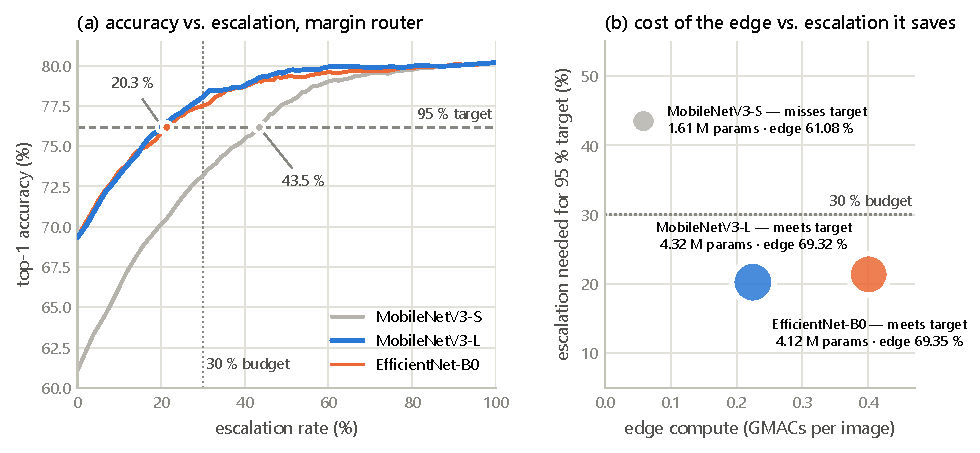
\includegraphics[width=\linewidth]{figures/fig_capacity.pdf}
\caption{Edge capacity and the escalation it requires. (a)~Accuracy versus escalation rate. (b)~Edge compute versus escalation needed for the 95\,\% target.}
\label{fig:offload}
\end{figure*}

The oracle curve in Fig.~\ref{fig:pareto} and the last column of
Table~\ref{tab:budgets} add a further observation. At 20\,\% escalation
the oracle reaches \RBudTwentyOracle\,\% with MobileNetV3-Large, \emph{above} the
always-cloud model: the edge and the cloud make partly different errors,
so a perfect router would beat both. The gap between the practical rules
and the oracle measures how much a better uncertainty signal could still
gain; it does not depend on the cloud model, which is unchanged.

\subsection{Accuracy--bandwidth trade-off}
\label{sec:res-headline}

Table~\ref{tab:headline} and Fig.~\ref{fig:pareto} place the operating
points on the bandwidth axis. Absolute traffic uses the measured mean payload $S=\RSKb$\,KB (Section~\ref{sec:bw}); the reduction factor does not depend on $S$. In the figure, the ring marks the operating point with the validation-calibrated threshold, the shaded region the pre-specified success criterion, and the light curve the oracle router, an upper bound for any escalation rule; the lower block of the table reads both routers' test curves at the same accuracy, for comparison only. With the validation-calibrated threshold,
margin escalation from MobileNetV3-Large reaches 75.82\,\% top-1 on the
test split --- 94.6\,\% of always-cloud accuracy --- while escalating
18.6\,\% of images: \ROffKbOp\,KB per diagnosis instead of \RSKb\,KB, a
5.38-fold reduction. On the validation split, where $\tau$ was set, the
rule meets the criterion by construction (95.0\,\% of cloud accuracy at
19.3\,\% escalation); the 0.4-point shortfall on test is the
generalisation gap of a threshold fixed in advance. Its size is what the
calibration's sampling variability predicts: recalibrating $\tau$ on
2\,000 bootstrap resamples of the validation split gives a test accuracy
between \RBootPctLo and \RBootPctHi\,\% of cloud accuracy (5th--95th
percentile; median \RBootPctMed\,\%) and an escalation rate between
\RBootEscLo and \RBootEscHi\,\%. A deployment that must meet the target
with high confidence can take the 95th percentile of the bootstrap
thresholds instead ($\tau=\RConsTau$): it then delivers \RConsPct\,\% of
cloud accuracy on test at \RConsEsc\,\% escalation, still a
\RConsRed-fold reduction. Read directly off the test curve, the 95\,\% line
is crossed at \REscNFLarge\,\% escalation (\ROffKbCross\,KB). Measured by
macro-F1, which weights the 89 classes equally, the operating point
delivers \RMfOp\,\% against \RMfEdge\,\% for the edge alone and
\RMfCloud\,\% for always-cloud, the same ordering as top-1.
The curve is
markedly concave: the first escalated images are the most valuable.
Escalating 30\,\% of images already closes \RGapClosedThirty\,\% of the gap between edge
and cloud accuracy (Table~\ref{tab:budgets}), so the last fifth of that
gap costs the remaining 70\,\% of the traffic. Table~\ref{tab:budgets} shows that the three scalar signals are
within \RBudSpread points of each other at every budget; we adopt the
margin because it ties for best at the target and is the simplest to
interpret.

\begin{table}[!htbp]
\centering
\caption{Operating points on the PlantWild test split (offline).}
\label{tab:headline}
\small
\begin{tabular}{@{}L{0.40\linewidth}rrrr@{}}
\toprule
\textbf{Operating point} & \textbf{KB/img} & \textbf{Escal.} & \textbf{Top-1} & \textbf{\% cloud} \\
\midrule
Edge only (MobileNetV3-L)                  &   0.0 &   0\,\% & 69.32\,\% &  86.5\,\% \\
\textbf{Margin escalation, $\tau{=}0.138$ calibrated on validation} & \textbf{\ROffKbOp} & \textbf{18.6\,\%} & \textbf{75.82\,\%} & \textbf{94.6\,\%} \\
Always-cloud                                & \RSKb & 100\,\%  & 80.17\,\% & 100\,\% \\
\midrule
\multicolumn{5}{@{}l}{\emph{Test curves read at 95\,\% of cloud accuracy}} \\
Margin escalation                           & \ROffKbCross &  \REscNFLarge\,\% & \RAccNFLarge\,\% &  \RPctNFLarge\,\% \\
Cloud-supervised verifier                   & \ROffKbVer &  \RVerEscNF\,\% & \RVerAccNF\,\% &  \RPctNFLarge\,\% \\
\bottomrule
\end{tabular}
\end{table}

\begin{figure*}[!htbp]
\centering
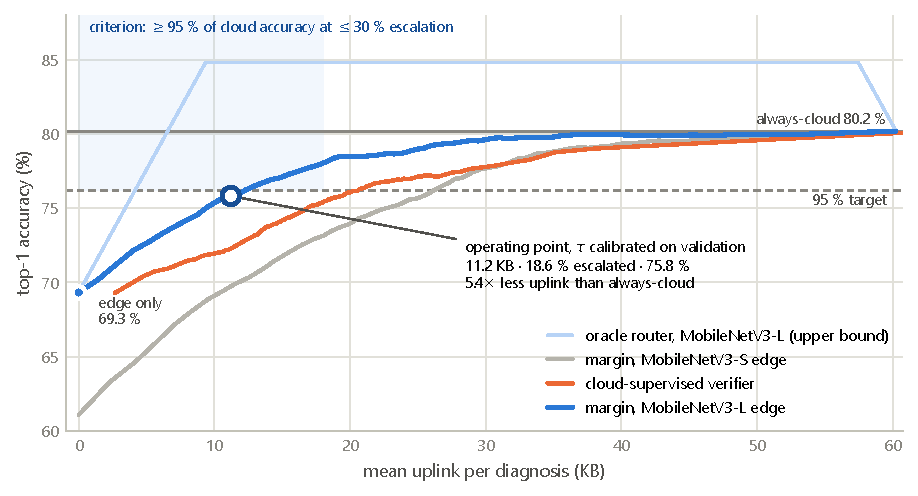
\includegraphics[width=\linewidth]{figures/fig_pareto.pdf}
\caption{Accuracy versus mean uplink per diagnosis (offline, test split).}
\label{fig:pareto}
\end{figure*}

\begin{figure*}[!htbp]
\centering
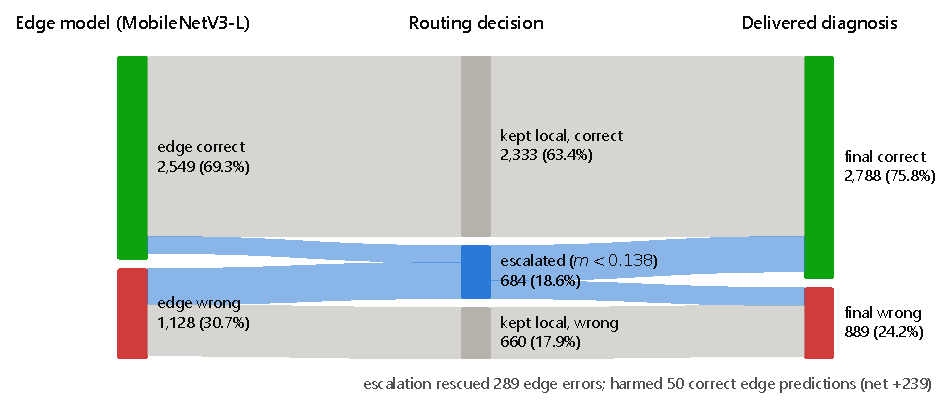
\includegraphics[width=\linewidth]{figures/fig_flow.pdf}
\caption{Flow of the 3\,677 test images at the calibrated threshold.}
\label{fig:flow}
\end{figure*}

Figure~\ref{fig:flow} follows every test image through the system. Band widths are proportional to image counts, and escalated images are drawn in blue. Of
the 684 escalated images, 468 (68\,\%) were edge errors, so the margin
spends uplink overwhelmingly where it is needed; the cloud rescues 289 of
them and overturns 50 correct edge predictions, a net gain of 239
diagnoses. The figure also shows the limit of any edge-side signal: 660
edge errors are made with a confident margin and never leave the farm.

\begin{figure*}[!htbp]
\centering
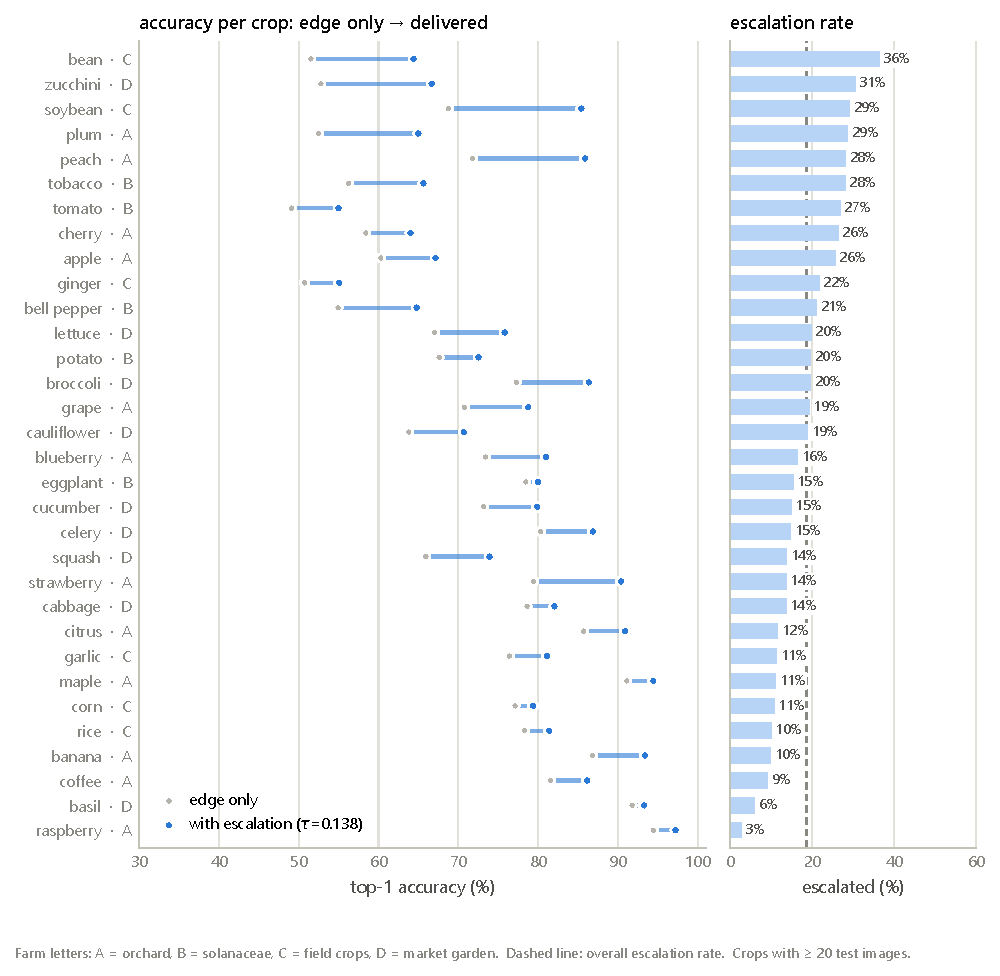
\includegraphics[width=\linewidth]{figures/fig_crops.pdf}
\caption{Per-crop accuracy before and after escalation, and per-crop escalation rate.}
\label{fig:crops}
\end{figure*}

The rule also adapts across crops without any per-crop tuning
(Fig.~\ref{fig:crops}). The figure shows, per crop, accuracy before and after escalation and the share of images escalated; the letters give each crop's farm in the emulation (Section~\ref{sec:fleet}). Escalation ranges from 3\,\% of raspberry images
to 36\,\% of bean images, and it is strongly anti-correlated with the edge
model's accuracy on the crop (Pearson $r=-0.85$): bandwidth flows to the
crops the edge finds hardest, which are also those that gain most ---
soybean (+16.7 points), peach (+14.1), zucchini (+13.9) and bean
(+12.9).

\begin{table}[!htbp]
\centering
\caption{Top-1 accuracy of MobileNetV3-L escalation at fixed escalation
budgets, by signal.}
\label{tab:budgets}
\small
\begin{tabular}{@{}rrrrr@{}}
\toprule
\textbf{Escalation} & \textbf{Max.\ probability} & \textbf{Margin} & \textbf{Entropy} & \textbf{Oracle} \\
\midrule
  5\,\% & \RBudFiveMaxP & \RBudFiveMargin & \RBudFiveEnt & \RBudFiveOracle \\
10\,\% & \RBudTenMaxP & \RBudTenMargin & \RBudTenEnt & \RBudTenOracle \\
15\,\% & \RBudFifteenMaxP & \RBudFifteenMargin & \RBudFifteenEnt & \RBudFifteenOracle \\
20\,\% & \RBudTwentyMaxP & \RBudTwentyMargin & \RBudTwentyEnt & \RBudTwentyOracle \\
25\,\% & \RBudTwentyFiveMaxP & \RBudTwentyFiveMargin & \RBudTwentyFiveEnt & \RBudTwentyFiveOracle \\
30\,\% & \RBudThirtyMaxP & \RBudThirtyMargin & \RBudThirtyEnt & \RBudThirtyOracle \\
\bottomrule
\end{tabular}
\end{table}

\subsection{A cloud-supervised verifier does not pay for itself}
\label{sec:res-verifier}

If edge-side signals are bounded by what the edge knows, a router that
is trained with the cloud's answers might do better. It does not
(Table~\ref{tab:auc}, Fig.~\ref{fig:verifier}). The best verifier scores
an AUC of 0.731 for identifying useful escalations, below the scalar
$1-m(x)$ at 0.810. On the bandwidth axis the verifier is dominated twice
over: it needs more escalations for the same accuracy (\RVerEscNF\,\% versus
\REscNFLarge\,\%) and it adds its 2.67\,KB message to every image. From
Eq.~\eqref{eq:bw}, merely breaking even would require the verifier to
escalate $M/S \approx \RVerifierBreakEven$ points \emph{fewer} images
than the margin rule; it escalates \RVerExtra points more. The tax grows as
payloads shrink: the more efficiently escalated images are encoded, the
larger an always-on message is relative to them. The verifier's
ranking also generalises poorly: the best target reaches an AUC of
\RVerValAuc on its held-out validation images but \RVerAuc on test,
the signature of a 1\,372-dimensional input fitted on 1\,820 images. On
this evidence the embedding carries no routing information beyond what
the edge posterior already exposes for free.

Could the scalar signals themselves be improved? The edge models are
trained with focal loss and label smoothing, which change the scale of
their softmax, so we also calibrated the posterior by temperature
scaling \citep{guo2017calibration} on the validation split
($T=\RTemp$; expected calibration error on test \REceRaw before and
\REceScaled after) and tried the margin between the two largest logits.
Every variant is calibrated by the same rule and evaluated on test
(Table~\ref{tab:auc}). For the original edge model, none improves on the
plain margin by more than a few tenths of a point of escalation; for the
distilled model of Section~\ref{sec:res-teacher}, the maximum
probability needs 1.4 points less escalation than the margin. The
differences between scalar signals are small compared with those between
edge models, which is why we keep the pre-specified margin rule.

\begin{table}[!htbp]
\centering
\caption{Escalation signals: ranking quality and escalation needed.}
\label{tab:auc}
\small
\setlength{\tabcolsep}{4pt}
\begin{tabular}{@{}lrrrr@{}}
\toprule
 & \multicolumn{2}{c}{\textbf{Original edge}} & \multicolumn{2}{c}{\textbf{Distilled edge}} \\
\cmidrule(lr){2-3}\cmidrule(l){4-5}
\textbf{Signal} & \textbf{AUC} & \textbf{Esc.\ @95\,\%} & \textbf{AUC} & \textbf{Esc.\ @95\,\%} \\
\midrule
$1 - $ margin (deployed)          & \RSigMarginAuc & \RSigMarginEsc\,\% & \RSigKdMarginAuc & \RSigKdMarginEsc\,\% \\
\quad temperature-scaled           & \RSigMarginTAuc & \RSigMarginTEsc\,\% & \RSigKdMarginTAuc & \RSigKdMarginTEsc\,\% \\
$1 - $ maximum probability        & \RSigMaxPAuc & \RSigMaxPEsc\,\% & \RSigKdMaxPAuc & \RSigKdMaxPEsc\,\% \\
\quad temperature-scaled           & \RSigMaxPTAuc & \RSigMaxPTEsc\,\% & \RSigKdMaxPTAuc & \RSigKdMaxPTEsc\,\% \\
Entropy                           & \RSigEntAuc & \RSigEntEsc\,\% & \RSigKdEntAuc & \RSigKdEntEsc\,\% \\
\quad temperature-scaled           & \RSigEntTAuc & \RSigEntTEsc\,\% & \RSigKdEntTAuc & \RSigKdEntTEsc\,\% \\
$-$(logit margin)                 & \RSigLogitAuc & \RSigLogitEsc\,\% & \RSigKdLogitAuc & \RSigKdLogitEsc\,\% \\
Cloud-supervised MLP verifier     & \RVerAuc & \RVerEscNF\,\% & --- & --- \\
\bottomrule
\end{tabular}
\end{table}

\begin{figure*}[!htbp]
\centering
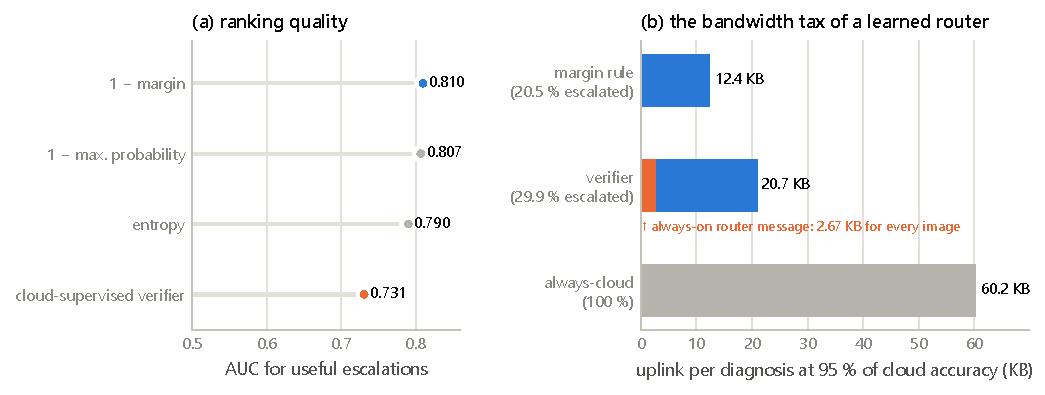
\includegraphics[width=\linewidth]{figures/fig_tax.pdf}
\caption{Cloud-supervised verifier versus scalar signals. (a)~Ranking quality (AUC). (b)~Uplink per diagnosis at 95\,\% of cloud accuracy.}
\label{fig:verifier}
\end{figure*}

\subsection{The ensemble as a teacher for the edge model}
\label{sec:res-teacher}
Section~\ref{sec:res-capacity} showed that edge capacity sets the
operating point. A more capable edge model need not be a larger one: the
cloud ensemble can teach it. We tested this in two ways
(Table~\ref{tab:teacher}). Both edge models are evaluated from the same
per-image predictions as Table~\ref{tab:headline}, with thresholds
calibrated on validation by the rule of Section~\ref{sec:router}.

\paragraph{Distillation before deployment} We retrained MobileNetV3-Large
with the recipe and split of Section~\ref{sec:edge}, adding to the loss the
Kullback--Leibler divergence to the ensemble's class probabilities on each
training image \citep{hinton2015distilling} (temperature 2, weight 0.5).
The probabilities come from the backbone features already computed for the
training split, so the teacher adds no inference cost, and the distilled
model keeps the architecture and on-device latency of the original. On its
own it reaches \RKdEdgeAcc\,\% top-1, against \RBaseEdgeAcc\,\% before
distillation. With its threshold recalibrated on validation by the same
rule (Section~\ref{sec:router}; $\tau=\RKdTau$), it escalates
\RKdEsc\,\% of test images instead of \RBaseEsc\,\% while delivering
\RKdPct\,\% of cloud accuracy, so uplink traffic falls \RKdRed-fold
instead of \RBaseRed-fold; on the test curve the 95\,\% target is reached
at \RKdEscNF\,\% escalation instead of \RBaseEscNF\,\%. Part of the
recalibrated model's saving comes from accepting slightly lower accuracy
(\RKdPct\,\% of cloud accuracy against \RBasePct\,\%), but most of it does
not: to match the original model's 75.82\,\%, the distilled model needs
\RIsoEsc\,\% escalation instead of 18.6\,\%, a \RIsoRed-fold reduction
instead of \RBaseRed-fold. The gain costs nothing at run time and needs
nothing the system does not already have: a stronger edge model obtained
from the cloud model itself. Section~\ref{sec:res-improved} confirms it
on the devices.

\paragraph{Closing the loop after deployment} Every escalated image
returns with the ensemble's verdict, a training signal the farm receives
for free. To test whether it can keep improving the deployed edge model,
we split the test set per class into a first ``week'' of about
\RLoopNWeek images, whose \RLoopNEsc escalated images are used to
fine-tune the deployed model, and a second week of the remaining images
for evaluation, and repeated the experiment over \RLoopParts random
partitions. Fine-tuning runs for eight short epochs (AdamW, learning rate
$10^{-4}$ with 10\,\% warm-up and cosine decay, the loss of the
distillation recipe), each mixing the escalated images, repeated four
times, with 2\,000 rehearsal images drawn from the training split by the
original training's class-balanced sampler; the threshold stays at the
deployed $\tau$. Because further fine-tuning perturbs a trained model by
itself, the reference for the escalated images is a control that
fine-tunes on rehearsal images only: it needs \RLoopCtlVsNone{}\,$\pm$\,\RLoopCtlVsNoneSd
points more escalation than the unchanged model, consistently across
partitions. Against this control, one week of escalations did not
improve the edge model, whatever labels the escalated images carried
(Table~\ref{tab:teacher}; differences in escalation @95\,\%, mean $\pm$
standard deviation over partitions): \RLoopHardVsCtl{}\,$\pm$\,\RLoopHardVsCtlSd
points with the ensemble's top-1 labels, \RLoopSoftVsCtl{}\,$\pm$\,\RLoopSoftVsCtlSd with
its probabilities, \RLoopSoftConfVsCtl{}\,$\pm$\,\RLoopSoftConfVsCtlSd with its
probabilities on confident escalations only, and \RLoopOracleVsCtl{}\,$\pm$\,\RLoopOracleVsCtlSd
even with farmer-confirmed true labels. The fixed-threshold columns show
the mechanism: the models fine-tuned on escalations escalate fewer images
at $\tau$ than the control but deliver lower accuracy, so they become
more confident on the hard cases they were shown without becoming more
often right. The \RLoopNEsc images --- about four per class, and the
hardest the edge sees --- are memorised rather than generalised from by a
model trained on 11\,778 images of the same distribution. The value of
the loop therefore lies in accumulating escalations over many weeks and
in adapting to farms whose images differ from the training data, which
an in-distribution benchmark cannot show; distilling the ensemble before
deployment is, by contrast, an immediate gain.

\begin{table}[!htbp]
\centering
\caption{The ensemble as a teacher: distillation and one-week loop pilot.}
\label{tab:teacher}
\footnotesize
\setlength{\tabcolsep}{3pt}
\begin{tabular}{@{}L{0.30\linewidth}rrrrr@{}}
\toprule
\textbf{Edge model} & \textbf{Edge} & \textbf{Escal.} & \textbf{Top-1} & \textbf{Uplink} & \textbf{Escal.} \\
 & \textbf{top-1} & & \textbf{(\% cloud)} & \textbf{reduction} & \textbf{@95\,\%} \\
\midrule
Original MobileNetV3-L      & \RBaseEdgeAcc\,\% & \RBaseEsc\,\% & \RBaseAcc\,\% (\RBasePct) & \RBaseRed & \RBaseEscNF\,\% \\
\textbf{Distilled from the ensemble} & \textbf{\RKdEdgeAcc\,\%} & \textbf{\RKdEsc\,\%} & \textbf{\RKdAcc\,\% (\RKdPct)} & \textbf{\RKdRed} & \textbf{\RKdEscNF\,\%} \\
\midrule
\multicolumn{6}{@{}l}{\emph{Loop pilot, week 2, mean of \RLoopParts partitions; \RLoopNEsc escalations labelled by}} \\
No update                   & \RLoopNoneEdge\,\% & \RLoopNoneEscTau\,\% & \RLoopNoneAccTau\,\% (\RLoopNonePct) & \RLoopNoneRed & \RLoopNoneEsc{}\,$\pm$\,\RLoopNoneEscSd\,\% \\
No new images (control)     & \RLoopReplayEdge\,\% & \RLoopReplayEscTau\,\% & \RLoopReplayAccTau\,\% (\RLoopReplayPct) & \RLoopReplayRed & \RLoopReplayEsc{}\,$\pm$\,\RLoopReplayEscSd\,\% \\
Ensemble, top-1 label       & \RLoopHardEdge\,\% & \RLoopHardEscTau\,\% & \RLoopHardAccTau\,\% (\RLoopHardPct) & \RLoopHardRed & \RLoopHardEsc{}\,$\pm$\,\RLoopHardEscSd\,\% \\
Ensemble, probabilities     & \RLoopSoftEdge\,\% & \RLoopSoftEscTau\,\% & \RLoopSoftAccTau\,\% (\RLoopSoftPct) & \RLoopSoftRed & \RLoopSoftEsc{}\,$\pm$\,\RLoopSoftEscSd\,\% \\
Ensemble, confident only (\RLoopConfN) & \RLoopSoftConfEdge\,\% & \RLoopSoftConfEscTau\,\% & \RLoopSoftConfAccTau\,\% (\RLoopSoftConfPct) & \RLoopSoftConfRed & \RLoopSoftConfEsc{}\,$\pm$\,\RLoopSoftConfEscSd\,\% \\
True label (farmer)         & \RLoopOracleEdge\,\% & \RLoopOracleEscTau\,\% & \RLoopOracleAccTau\,\% (\RLoopOraclePct) & \RLoopOracleRed & \RLoopOracleEsc{}\,$\pm$\,\RLoopOracleEscSd\,\% \\
\bottomrule
\end{tabular}
\end{table}

\subsection{On-device latency and energy}
\label{sec:res-latency}

Table~\ref{tab:latency} reports latencies measured on the devices. Each measurement is for a single image (batch size 1); deployment values are medians over the baseline deployment. On
the Raspberry Pi~5, MobileNetV3-Large runs in 65.5\,ms per image (fp32,
$224{\times}224$, mean of 200 runs after warm-up, no thermal throttling).
A FLOPs-based projection from the device's nominal throughput had
predicted 32.1\,ms; the measured figure is about twice as slow, which
illustrates why projected latencies should not stand in for
measurements on embedded targets. On the Jetson Nano the three backbones
take \RMsDinoTwo, \RMsDinoThree and \RMsClip\,ms, so an escalated image costs
\RCloudS\,s of cloud computation including preprocessing and the head;
loading the three backbones adds \RLoadS\,s per batch, shared by all
images in it. Because escalation is deferred, none of this is on the
farmer's path to a diagnosis: the farm answers in a median of
\RAnswerMs\,ms over all images (95\,\% within
\RAnswerPNinetyFiveMs\,ms) --- \RAnswerLocalMs\,ms for images answered
locally and \RAnswerEscMs\,ms for escalated images, whose answer waits
for the upload to the cloud queue (Section~\ref{sec:edge-node}) --- and
the ensemble's confirmation arrives with the next batch. Figure~\ref{fig:fleet-latency}a shows this time to the farmer's answer for every image of the baseline deployment: escalated images are answered by the edge as soon as their upload to the cloud queue is acknowledged, and confirmed by the cloud at the next batch. Figure~\ref{fig:fleet-latency}b breaks the cost of one escalation into edge inference on the Pi, upload and Nano compute, excluding the wait for the next batch and the per-batch model loading.

Energy was measured on both devices. On the Pi, the power-management IC
reports the voltage and current of every supply rail; over \RPiN edge
inferences the SoC and memory rails drew \RPiLoadW\,W on average
(\RPiIdleW\,W at idle), or \RPiEImgJ\,J per image (\RPiEIncrJ\,J above
idle). These rails exclude peripherals powered directly from the 5\,V
input, so the figure is a lower bound for the board. On the Nano, an
escalated image costs \RNanoEImgJ\,J at the board's input
(Section~\ref{sec:batch}). A diagnosis under selective escalation therefore
costs \RSysEJ\,J of device energy (every image on the edge, \REscRate of
them also on the cloud node), against \RSysCloudEJ\,J when every image is
sent to the same cloud node: \RSysERatio times less, in line with the
bandwidth saving.

\begin{table}[!htbp]
\centering
\caption{Latency measured on the embedded devices.}
\label{tab:latency}
\small
\begin{tabular}{@{}L{0.19\linewidth}L{0.56\linewidth}r@{}}
\toprule
\textbf{Device} & \textbf{Stage} & \textbf{Latency} \\
\midrule
Raspberry Pi~5 & MobileNetV3-L forward (fp32, 224\,px), 200 runs & 65.5\,ms \\
               & \quad FLOPs-based projection, for reference & \emph{32.1\,ms} \\
               & edge inference incl.\ preprocessing (deployment) & \REdgeMs\,ms \\
               & answer on the farm, end to end (deployment)     & \RAnswerMs\,ms \\
               & energy per image (SoC and memory rails)     & \RPiEImgJ\,J \\
\midrule
Jetson Nano    & DINOv2-L/14, 336\,px (4 chunk engines, fp16) & \RMsDinoTwo\,ms \\
               & DINOv3-L/16, 336\,px (4 chunk engines, fp32) & \RMsDinoThree\,ms \\
               & CLIP-L/14, 224\,px (4 chunk engines, fp32)   & \RMsClip\,ms \\
               & cloud compute per escalated image (deployment)   & \RCloudS\,s \\
               & loading the three backbones, per batch (deployment) & \RLoadS\,s \\
               & energy per escalated image (board input)    & \RNanoEImgJ\,J \\
\midrule
Network        & escalation upload to the cloud queue (deployment) & \RNetMs\,ms \\
\bottomrule
\end{tabular}
\end{table}

\subsection{Seven-day, four-farm emulated deployment}
\label{sec:res-fleet}

Over the emulated week of the baseline deployment, the four farms submitted \RNImg images, and the
edge escalated \RNEsc of them (\REscRate) --- the rate predicted offline
for the same images at the same threshold (18.6\,\%), as expected from
the edge node's agreement with the offline model (Table~\ref{tab:fidelity}).
The farms uploaded \RUpMB\,MB in total, against \RCloudOnlyMB\,MB had
every image been sent with the same payload: a \RReduction-fold reduction
in the bytes actually uploaded (Fig.~\ref{fig:fleet}). The figure shows the escalations per simulated hour, by farm, with nights shaded, and the cumulative uploaded bytes against the same images uploaded with the same payload by an always-cloud design; its green curve is the distilled deployment (Section~\ref{sec:res-improved}). The offline model
of Eq.~\eqref{eq:bw} predicted \ROffKbOp\,KB per diagnosis; the devices
measured \RKbPerImg. The system delivered
\RAcc correct diagnoses, against \REdgeAcc for the edge alone. On the
escalated images, the Nano's ensemble was correct on \RCloudAccEsc of
them; the workstation's offline predictions for the same images, which
like all offline results are computed from the original full-resolution
files, reach \ROfflineCloudAccEsc, and the two agree on \RCloudAgreeFleet
images (\RCloudAgreeFleetPct). Running the workstation's reference
pipeline on both inputs separates the two causes: on these images it is
correct on \RRefEscFullAcc from the original files and on \RRefEscPayAcc
from the 448\,px payload, so the payload itself does not cost accuracy,
and the Nano agrees with it on \RPayNanoAgree images, the remainder being
the decoder difference of Section~\ref{sec:verify}. The on-device
deviation changes individual diagnoses but not accuracy. The cloud node processed \RNFlush batches of
\RBatchMed images at the median, never received more than \RMaxPerHour
escalations in a simulated hour, and confirmed every escalated image on
the day it was captured (at most \RDelayMax simulated hours later). The
whole emulation took \RWallMin minutes of wall-clock time, almost all of it
spent on cloud computation.

The farms behave differently (Table~\ref{tab:fleet},
Fig.~\ref{fig:fleet-offline}): \RFarmMaxName escalated most often
(\RFarmMaxEsc) and \RFarmMinName least (\RFarmMinEsc), in line with the
per-farm rates predicted offline from the margins of the same images. A
single global threshold therefore translates into farm-specific uplink
budgets that follow how hard each farm's crops are for the edge model,
which a deployment can monitor and, if needed, tune per farm. Delivered
accuracy also differs between farms, from \RFarmBAcc (solanaceae) to
\RFarmDAcc (market garden), but mostly because the farms' crops differ in
difficulty for the cloud model too: measured against each farm's own
always-cloud accuracy (last column of Table~\ref{tab:fleet}), every farm
receives between \RFarmCPctCloud and \RFarmDPctCloud of what the ensemble
alone would deliver, solanaceae included (\RFarmBPctCloud).
Figure~\ref{fig:console} shows the operations console at the end of the baseline deployment. It displays the simulated clock and node status, fleet indicators, escalations per simulated hour, per-farm cards, the topology, latency by stage and a feed of the most recent diagnoses.

\begin{table}[!htbp]
\centering
\caption{Per-farm results of the baseline deployment.}
\label{tab:fleet}
\footnotesize
\setlength{\tabcolsep}{3pt}
\begin{tabular}{@{}lrrrrrrr@{}}
\toprule
\textbf{Farm} & \textbf{Images} & \textbf{Escal.} & \textbf{Upload} & \textbf{Always-} & \textbf{Reduc-} & \textbf{Top-1} & \textbf{Cloud} \\
 & & & \textbf{(MB)} & \textbf{cloud (MB)} & \textbf{tion} & & \textbf{top-1} \\
\midrule
A --- orchard        & 1\,360 & \RFarmAEsc & \RFarmAUp & \RFarmACloud & \RFarmARed{}$\times$ & \RFarmAAcc & \RFarmACeil \\
B --- solanaceae     &   701 & \RFarmBEsc & \RFarmBUp & \RFarmBCloud & \RFarmBRed{}$\times$ & \RFarmBAcc & \RFarmBCeil \\
C --- field crops    &   707 & \RFarmCEsc & \RFarmCUp & \RFarmCCloud & \RFarmCRed{}$\times$ & \RFarmCAcc & \RFarmCCeil \\
D --- market garden  &   909 & \RFarmDEsc & \RFarmDUp & \RFarmDCloud & \RFarmDRed{}$\times$ & \RFarmDAcc & \RFarmDCeil \\
\midrule
All farms            & 3\,677 & \REscRate & \RUpMB & \RCloudOnlyMB & \RReduction{}$\times$ & \RAcc & 80.2\,\% \\
\bottomrule
\end{tabular}
\end{table}

\begin{figure*}[!htbp]
\centering
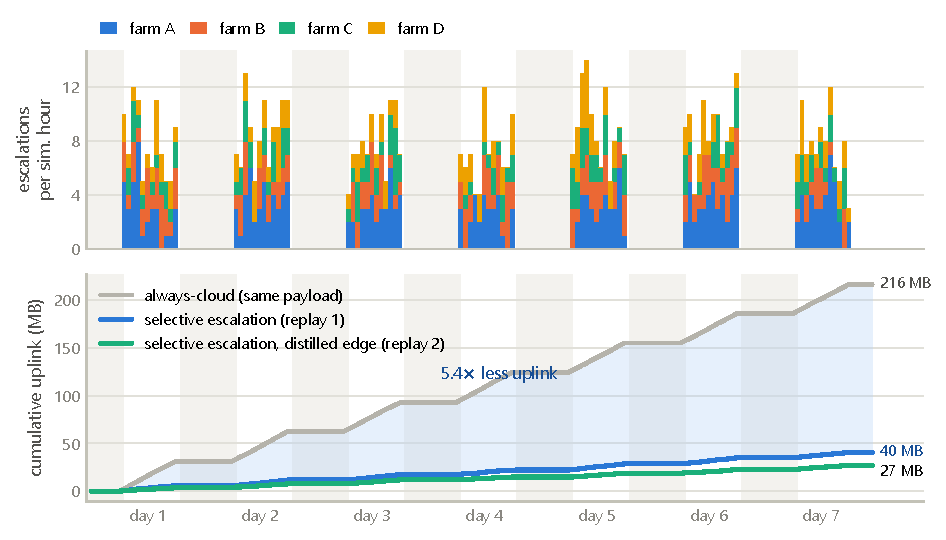
\includegraphics[width=\linewidth]{figures/fig_fleet_timeline.pdf}
\caption{Escalations per simulated hour and cumulative uplink over the seven-day emulated deployments.}
\label{fig:fleet}
\end{figure*}

\begin{figure*}[!htbp]
\centering
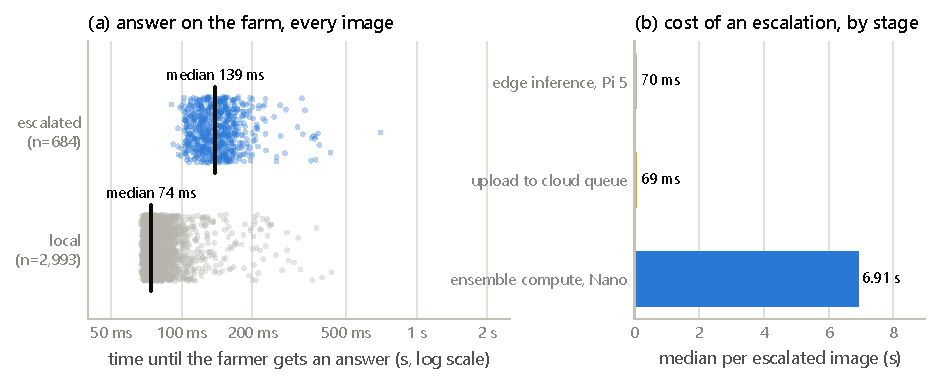
\includegraphics[width=\linewidth]{figures/fig_fleet_latency.pdf}
\caption{Measured latency during the baseline deployment. (a)~Time to the farmer's answer, per image. (b)~Median cost of one escalation, by stage.}
\label{fig:fleet-latency}
\end{figure*}

\begin{figure}[!htbp]
\centering
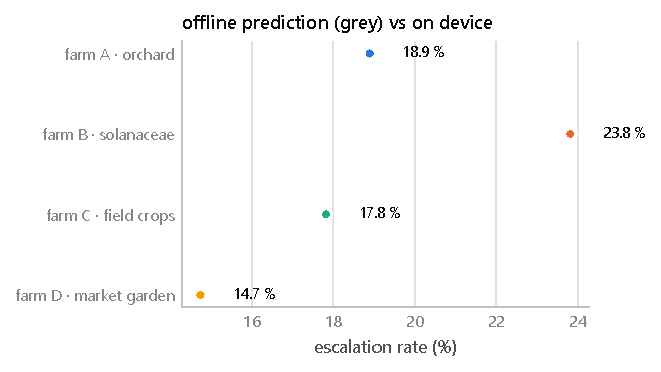
\includegraphics[width=\linewidth]{figures/fig_fleet_vs_offline.pdf}
\caption{Escalation rate per farm: offline prediction and on-device measurement.}
\label{fig:fleet-offline}
\end{figure}

\begin{figure*}[!htbp]
\centering
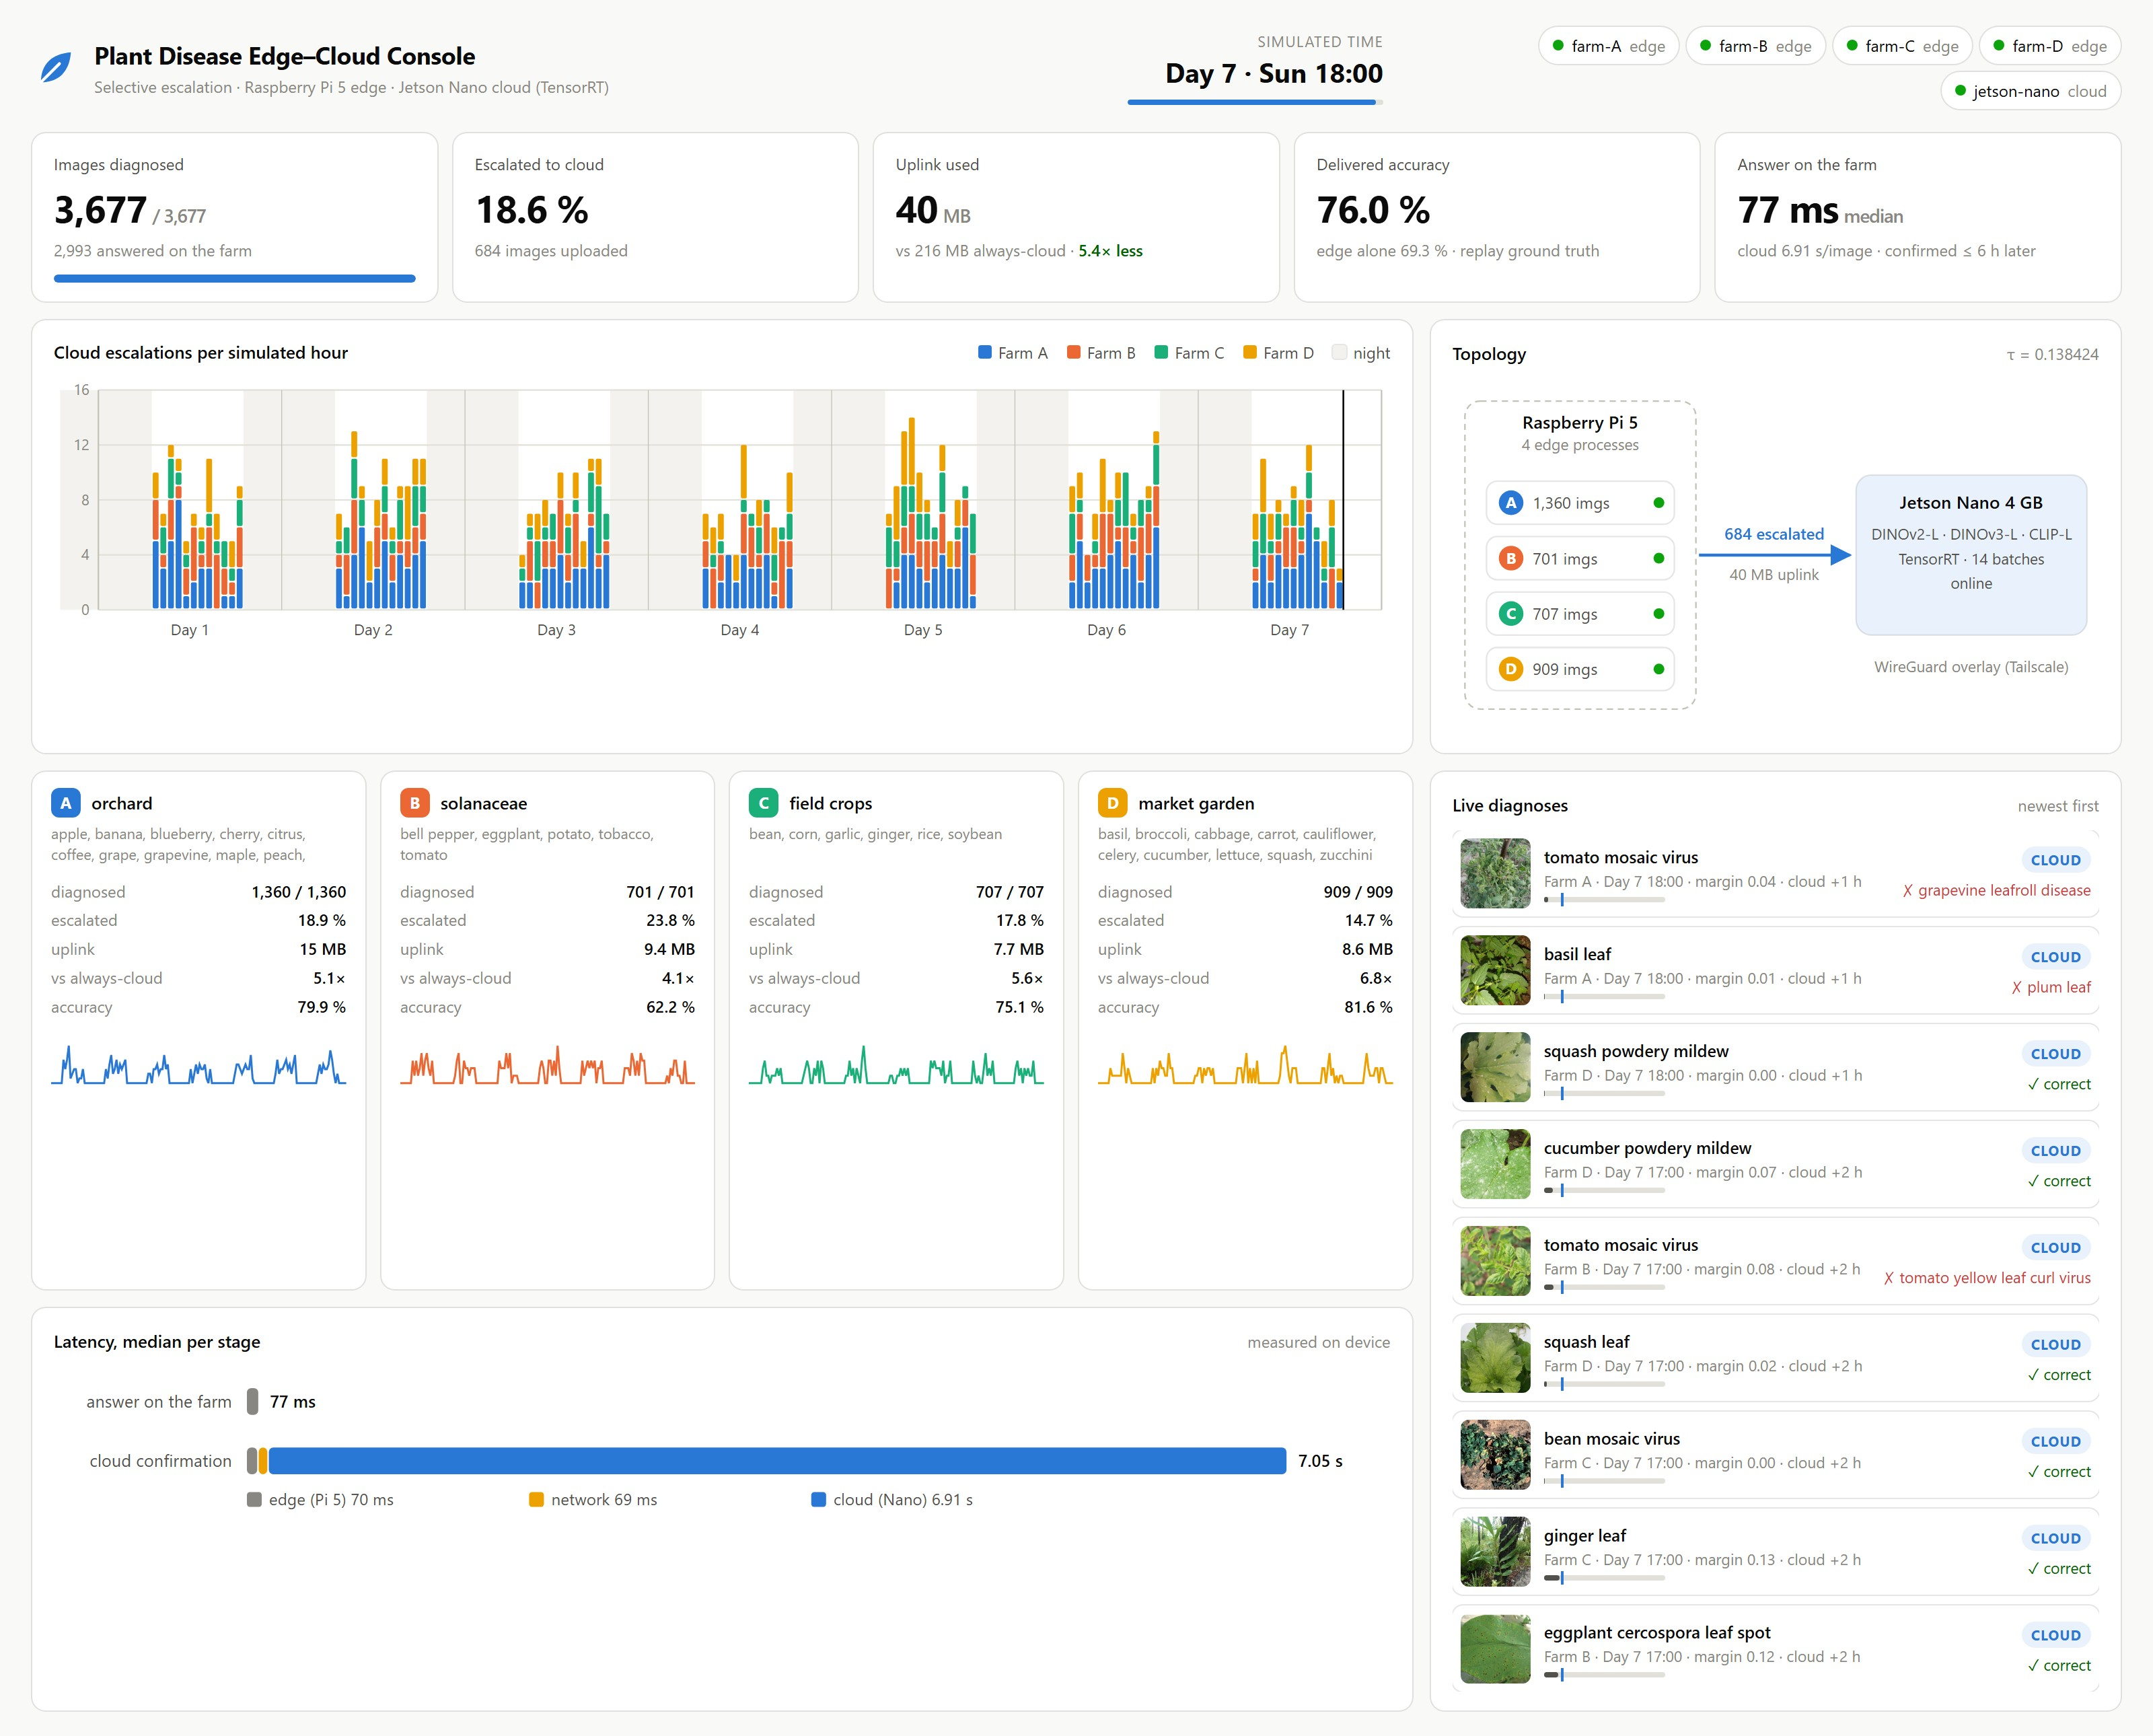
\includegraphics[width=\linewidth]{figures/fig_console.jpg}
\caption{Operations console during the baseline deployment.}
\label{fig:console}
\end{figure*}

\subsection{Distilled configuration on the devices}
\label{sec:res-improved}
The ensemble's most effective contribution to the edge is made once,
before deployment. Distillation (Section~\ref{sec:res-teacher}) leaves
the edge model's architecture, size and on-device cost unchanged, so we
deployed the distilled MobileNetV3-Large on the same devices, together
with the other improvement found after the baseline deployment, CLIP in
fp16 (Section~\ref{sec:port}); neither changes an interface
(\mbox{\ref{app:adaptations}}, item~C4). We then repeated the seven-day
emulation with identical images, schedule, payload and batch times. The
distilled model's threshold was recalibrated on validation by the rule
of Section~\ref{sec:router} ($\tau=\RImpTau$), and before the run the
deployed edge reproduced the distilled model's offline predictions on
300 of 300 test images. Table~\ref{tab:replays} compares the two
deployments.

\paragraph{Bandwidth} The edge escalated \RImpNEsc images
(\RImpEscRate, against the offline prediction of \RImpOffEscRate), and
the farms uploaded \RImpUpMB\,MB instead of \RUpMB\,MB: \RImpKbPerImg per
diagnosis, an \RImpReduction-fold reduction against always-cloud measured
on the devices, compared with \RReduction-fold for the original edge
model (Fig.~\ref{fig:fleet}). Every farm saved more than in the baseline
deployment, from \RImpFarmBRed-fold (solanaceae) to \RImpFarmDRed-fold
(market garden). Delivered accuracy was \RImpAcc, against \RAcc: both
thresholds target 95\,\% of cloud accuracy on validation, so the stronger
edge model spends its gain on bandwidth rather than on accuracy. The gain
does not depend on that choice. At equal accuracy the distilled model
still escalates far less: offline, it matches the original model's
delivered accuracy (75.82\,\%) at \RIsoEsc\,\% escalation instead of
18.6\,\%, a \RIsoRed-fold reduction instead of 5.4-fold, and the baseline
deployment's \RAcc at \RIsoRunEsc\,\% (\RIsoRunRed-fold).

\paragraph{Cost on the devices} Two changes coincide in this deployment,
and they act on different quantities. Distillation changes only how many
images are escalated; the edge model's latency is unchanged (median
answer \RImpAnswerMs\,ms against \RAnswerMs\,ms). fp16 CLIP changes only
what an escalated image costs on the Nano: compute per escalated image
fell from \RCloudS to \RImpCloudS\,s and model loading per batch from
\RLoadS to \RImpLoadS\,s. The whole emulation took \RImpWallMin instead
of \RWallMin minutes of wall-clock time, a reduction in proportion to the
number of escalated images. On the Nano an escalated image costs
\RNanoEImgJ\,J with fp32 CLIP and \RNanoTwoEImgJ\,J with fp16 CLIP in
batches of 48, and \RNanoThreeFourEImgJ\,J in batches of
\RNanoThreeFourN, the median batch of this deployment
(\RNanoThreeFourRuns runs), so the smaller batches did not raise the
energy per image. A diagnosis therefore cost \RImpSysEThreeFourJ\,J of
device energy, against \RSysEJ\,J in the baseline deployment; at the
fp32-CLIP energy per escalated image it would have cost
\RImpSysEFpThirtyTwoJ\,J, so distillation accounts for nearly all of the
saving and fp16 CLIP for the rest. Against an always-cloud design on the
same cloud node, which spends \RNanoTwoEImgJ\,J on every image, the
distilled configuration uses \RImpSysERatio times less device energy per
diagnosis. The Nano's diagnoses agreed with the workstation's offline
predictions on \RImpCloudAgree escalated images.

\begin{table}[!htbp]
\centering
\caption{The two emulated deployments on the embedded testbed.}
\label{tab:replays}
\small
\begin{tabular}{@{}L{0.46\linewidth}rr@{}}
\toprule
 & \textbf{Baseline} & \textbf{Distilled} \\
\midrule
Edge model                               & original & distilled \\
CLIP precision on the Nano               & fp32 & fp16 \\
Threshold $\tau$ (calibrated on validation) & 0.138 & \RImpTau \\
\midrule
Images escalated                         & \REscRate & \RImpEscRate \\
Uploaded (always-cloud: \RCloudOnlyMB\,MB) & \RUpMB\,MB & \RImpUpMB\,MB \\
Uplink reduction                         & \RReduction{}$\times$ & \RImpReduction{}$\times$ \\
Uplink per diagnosis                     & \RKbPerImg & \RImpKbPerImg \\
Delivered top-1                          & \RAcc & \RImpAcc \\
Delivered macro-F1                       & \RMfRunOne\,\% & \RMfRunTwo\,\% \\
Edge model alone, top-1                  & \REdgeAcc & \RImpEdgeAcc \\
Uplink reduction at equal accuracy (offline) & \RBaseRed{}$\times$ & \RIsoRed{}$\times$ \\
\midrule
Answer on the farm, median               & \RAnswerMs\,ms & \RImpAnswerMs\,ms \\
Nano compute per escalated image, median & \RCloudS\,s & \RImpCloudS\,s \\
Model loading per batch, median          & \RLoadS\,s & \RImpLoadS\,s \\
Batches (median size)                    & \RNFlush{} (\RBatchMed) & \RImpNFlush{} (\RImpBatchMed) \\
Nano energy per escalated image          & \RNanoEImgJ\,J & \RNanoThreeFourEImgJ\,J \\
Device energy per diagnosis              & \RSysEJ\,J & \RImpSysEThreeFourJ\,J \\
Wall-clock time of the emulation         & \RWallMin\,min & \RImpWallMin\,min \\
Nano--workstation agreement, escalated images & \RCloudAgreeFleet & \RImpCloudAgree \\
\bottomrule
\end{tabular}
\end{table}

% =====================================================================
\section{Discussion}
\label{sec:discussion}
% =====================================================================

\paragraph{Strengthen the edge before engineering the router}
The most consequential design decision in our study was not the
escalation rule but the edge model. Moving from MobileNetV3-Small to
MobileNetV3-Large cost 2.7$\times$ the parameters and 3.8$\times$ the
operations --- still only 65.5\,ms on a Raspberry Pi~5 --- and halved
the escalation rate, whereas a learned edge-side router saved only two
points of escalation and a cloud-supervised one did worse than the
training-free scalar. Capacity can also be added without changing the
architecture: distilling the ensemble into the same MobileNetV3-Large cut
the calibrated escalation rate from \RBaseEsc to \RKdEsc\,\%
(Section~\ref{sec:res-teacher}), and on the devices from \REscRate to
\RImpEscRate, an \RImpReduction-fold uplink saving
(Section~\ref{sec:res-improved}). Our comparison covers convolutional
edge models, which are what runs efficiently on the Pi's CPU with stock
PyTorch; lightweight hybrid CNN--transformer models might align better
with a transformer teacher, and the same comparison would tell whether
they move the operating point further. The reason is
informational: an edge-side router can only re-express the edge model's
posterior, and the margin already summarises it well. The oracle shows
that substantial headroom remains (\RBudTwentyOracle\,\% at 20\,\% escalation), but
reaching it requires information the edge does not have; a cheaper path
to it is a stronger edge model.

\paragraph{What the bandwidth axis reveals}
Latency-centred evaluations treat an always-on router message as
negligible; on the bandwidth axis it is a fixed tax that a learned router
must earn back through fewer escalations. For field deployments on
metered cellular links the relevant figure is the uplink volume per farm
and month. At the measured \RKbPerImg per diagnosis, a farm capturing
\RImgPerDay images per day would upload \RMonthMB\,MB in a 30-day month,
against \RMonthCloudMB\,MB for always-cloud with the same payload, and
with the distilled edge model \RImpMonthMB\,MB; on a
\RUplinkMbps\,Mbit/s uplink an escalated image takes about \RUplinkS\,s to
transmit.

\paragraph{A cloud that fits on a farm}
Serving a 0.9-billion-parameter ensemble from a 4\,GB Jetson Nano shows
that the ``cloud'' in selective escalation need not be a data centre. A
cooperative, an extension office or a large farm can host the large
model locally, which keeps field images within the community's network,
removes the dependency on wide-area connectivity for the cloud tier, and
turns a recurring service cost into a one-off hardware cost. It does not
come for free. Each escalated image costs \RCloudS\,s of Nano compute, and
because the full ensemble does not fit in memory, the cloud tier must
work in batches; in the baseline deployment a batch of \RBatchMed images also paid
\RLoadS\,s to load the three backbones, and the board spends
\RNanoEImgJ\,J per escalated image (Section~\ref{sec:batch}). Selective
escalation is what makes this affordable: at 18--19\,\% escalation the
Nano sees one image in five, and at the distilled edge model's
\RImpEscRate one image in eight, whereas an always-cloud design would
multiply its workload, and its energy use, more than fivefold and
eightfold respectively. Beyond this study,
the port shows that hardware the software ecosystem has left behind can
still serve current foundation models, provided memory, precision and
fidelity are engineered explicitly; the same five principles apply to
other legacy accelerators that farms and cooperatives already own. The batched design suits scouting and monitoring workflows, in
which a confirmed diagnosis within hours is valuable but an instant one
is not required; the farmer always receives the edge's answer without
waiting for the ensemble. A node with more memory, such as an 8\,GB module, could keep
all engines resident and answer synchronously; the server implements this
mode, but we have not tested it.

\paragraph{Portability is more than the model} Two of the deviations we
measured did not come from the models at all. The edge server initially
resized images bicubically while the edge model had been trained with
bilinear resizing, and the Nano's older image library decodes JPEGs
differently (Section~\ref{sec:verify}). Both shifted predictions without
any error being raised. Verifying deployed nodes against offline
predictions image by image, as in Table~\ref{tab:fidelity}, is what
exposed them; we recommend the practice for any edge--cloud deployment.

\paragraph{Limitations}
Our study uses a single, if diverse, benchmark; PlantWild's class
balance and capture conditions may differ from a given region. The
escalation threshold is global; per-crop thresholds could equalise
accuracy across farms. The emulation compresses idle time and therefore
does not capture diurnal effects, power cycling or connectivity
outages, and its four farms share one physical Pi, so device-to-device
variability is not represented. Each edge model was trained once, so we
report no variance across training seeds for the edge models and the
distillation; the bootstrap of Section~\ref{sec:res-headline} covers the
variability of the calibrated threshold, and the loop pilot is repeated
over \RLoopParts random partitions. The escalation threshold is a point
estimate whose test result falls on either side of the target, and the
benchmark has no second field dataset with the same classes on which to
test it, so we do not claim a guarantee beyond PlantWild. In the
prototype the farmer's answer to an escalated image waits for the upload
to be acknowledged (Section~\ref{sec:edge-node}). The Pi's energy covers its SoC and
memory rails only and is therefore a lower bound. In our testbed the devices share a local
network, so measured network latencies are a best case for rural links;
transfer times on slower links follow directly from the measured byte
counts. The confirmation delay of the batched cloud tier is a design
parameter set in simulated time (two batches a day), not a measured
quantity; its compute and loading costs are measured. Finally, the
Nano's cloud pipeline deviates slightly from the workstation's, chiefly
through its older image library; Table~\ref{tab:fidelity} and the
deployment-wide agreement quantify the deviation.

% =====================================================================
\section{Conclusion}
\label{sec:conclusion}
% =====================================================================

Selective escalation reconciles the accuracy of foundation-model
ensembles with the connectivity of real farms. A MobileNetV3-Large edge
model that forwards an image only when its two leading hypotheses are
close --- with a threshold fixed on validation data --- retains 94.6\,\% of
a three-backbone ensemble's accuracy on held-out in-the-wild plant
disease images while uploading 5.4 times less data.
Edge-model capacity, not router complexity, sets this trade-off, and a
cloud-supervised verifier pays for its own message without improving
routing. The complete system runs on a Raspberry Pi~5 and an end-of-life
4\,GB Jetson Nano, made possible by a port that decouples the ensemble from
its framework and runs it one chunk engine at a time, at \RNanoEImgJ\,J
per escalated image; a seven-day, four-farm emulated deployment on that hardware
confirms the
offline trade-off: \REscRate of images escalated, uploaded bytes cut
\RReduction-fold, and \RAcc of diagnoses correct, with a median answer
time on the farm of \RAnswerMs\,ms and \RSysERatio times less device energy
per diagnosis than always-cloud. Distilling the ensemble into the edge
model, once and at no inference cost, raises the uplink saving measured
on the same devices from \RReduction- to \RImpReduction-fold
(\RImpKbPerImg per diagnosis) at \RImpAcc delivered accuracy --- and to
\RIsoRed-fold at unchanged accuracy --- while cutting device energy per
diagnosis from \RSysEJ to \RImpSysEThreeFourJ\,J. Future work will accumulate escalations over full seasons
to test whether the loop from cloud to edge improves farms whose images
differ from the training data, a gain one week of in-distribution
escalations could not show; it will also tune thresholds per crop and
study connectivity outages over full-length deployments.

% =====================================================================
\section*{CRediT authorship contribution statement}
\textbf{Youssef Natij, Hajar El Karch, Abdelkader Mezouari:}
Conceptualization, Methodology, Software,
Validation, Investigation, Formal analysis, Writing -- original draft,
Writing -- review \& editing. All authors contributed equally to the
conception, implementation, analysis and writing of this work.

\section*{Declaration of competing interest}
The authors declare that they have no known competing financial
interests or personal relationships that could have appeared to
influence the work reported in this paper.

\section*{Funding}
This research did not receive any specific grant from funding agencies
in the public, commercial, or not-for-profit sectors.

\section*{Data availability}
PlantWild is available from its authors \citep{wei2024plantwild} under
the terms of their release; this work does not redistribute its images.
Everything needed to reproduce the tables and figures of this paper is
in the project repository, \url{https://github.com/YouROS12/CloudOffEdge}:
the deployment code for the Raspberry Pi and the Jetson Nano, the porting
toolkit (chunked ONNX export, fp16 conversion, chunk-by-chunk TensorRT
build, chunk-major runtime), the fleet emulator and operations console, the
training, distillation, calibration and measurement scripts, the trained
edge models and cloud head, the per-image predictions, the per-image logs
of both emulated deployments, the activation, memory and power profiles, the TensorRT
verification reports and the sources of this manuscript.

\section*{Declaration of generative AI and AI-assisted technologies in the
manuscript preparation process}
During the preparation of this work the authors used Claude (Anthropic)
to assist with software development and with drafting and editing the
manuscript. After using this tool, the authors reviewed and edited the
content as needed and take full responsibility for the content of the
publication.

% =====================================================================
\appendix
\section{Software adaptations for embedded deployment}
\label{app:adaptations}
\setcounter{table}{0}\setcounter{figure}{0}\setcounter{equation}{0}
% Curated from deploy/ADAPTATIONS.md (the running log); its last section maps
% these item numbers to the log's own numbering. Keep both in sync.
% =====================================================================

The reference pipeline was developed on a workstation (Python~3.12,
PyTorch~2.11, \texttt{timm}~1.0.26, \texttt{open\_clip}~3.3.0). Running it
on the embedded testbed required the adaptations below, listed so that
the deployment can be reproduced on the same hardware generation. Each
adaptation was verified against the reference pipeline
(Table~\ref{tab:fidelity}).

{\small
\setlength{\tabcolsep}{4pt}
\begin{longtable}{@{}p{0.06\linewidth}L{0.39\linewidth}L{0.47\linewidth}@{}}
\caption{Software adaptations, by node.}\label{tab:adaptations}\\
\toprule
\textbf{\#} & \textbf{Problem and cause} & \textbf{Adaptation} \\
\midrule
\endfirsthead
\toprule
\textbf{\#} & \textbf{Problem and cause} & \textbf{Adaptation} \\
\midrule
\endhead
\bottomrule
\endfoot
\multicolumn{3}{@{}p{0.92\linewidth}}{\emph{Edge node --- Raspberry Pi 5, Debian 13, Python 3.13}} \\
A1 & The edge requirements originally pinned PyTorch 2.2 and NumPy 1.26, which have no Python 3.13 wheels for ARM64 (the workstation reference itself uses PyTorch~2.11). &
     Version-conditional pins (PEP~508 markers): original pins below 3.13, PyTorch 2.6 / NumPy 2.2 from 3.13. \\
A2 & One physical device must emulate several farms. &
     systemd template unit; one independent server process per farm with its own identifier and port. \\
A3 & Latency reported only as a total. &
     Edge reports its own inference time; the cloud reports per-backbone times; network time is the remainder. \\
A4 & A cloud outage would appear as a low escalation rate. &
     Escalation decisions logged separately from cloud success; failed escalations fall back to the edge label. \\
A5 & The edge server resized images bicubically, whereas the model was trained and evaluated with bilinear resizing, which shifts the margins. &
     Bilinear resizing restored; the deployed node reproduces the offline prediction on 300/300 test images. \\
A6 & Escalated images were uploaded at camera resolution (up to ${\sim}$6\,MB), although the cloud works at $\leq$336\,px. &
     Payload resized to a 448\,px shorter side, JPEG q90 (Table~\ref{tab:payload}); the always-cloud baseline uses the same payload. \\
A7 & A failed escalation was billed as uploaded bytes. &
     Bytes are counted only once the cloud acknowledges the image. \\
\midrule
\multicolumn{3}{@{}p{0.92\linewidth}}{\emph{Cloud node --- Jetson Nano 4\,GB, JetPack 4.6.1, Python 3.6, CUDA 10.2, TensorRT 8.2.1}} \\
B1 & The reference server needs Python $\geq$3.8 (PyTorch~2, \texttt{timm} for DINOv3), unavailable on JetPack~4. &
     Model decoupled from framework: ONNX export on the workstation, TensorRT engines built on the Nano, torch-free Python~3.6 server. \\
B2 & TensorRT~8.2 parses ONNX opsets up to 13. &
     Export at opset~13 with the TorchScript-based exporter. \\
B3 & Fused scaled-dot-product attention has no opset-13 mapping. &
     Explicit $\mathrm{softmax}(QK^\top/\sqrt{d})V$ substituted during export (mathematically identical). \\
B4 & The \texttt{nn.MultiheadAttention} fast path (CLIP) emits a fused operator with no ONNX mapping. &
     Fast path disabled during export. \\
B5 & DINOv2 bicubically resizes its position grid on every forward; TensorRT~8.2 has no cubic resize. &
     Input size is fixed, so the interpolated position embedding is computed once in PyTorch and stored as a constant. \\
B6 & DINOv3 recomputes its rotary position embedding from the input shape on every forward, and CLIP's reshapes emit dynamic shape arithmetic; both export as conditionals (\texttt{If}) and modulo operators. &
     Rotary embedding baked as a constant for the fixed $21{\times}21$ patch grid; remaining shape arithmetic constant-folded (onnx-simplifier); export rejected if an unsupported operator remains. \\
B7 & No PyTorch/torchvision in the serving process. &
     Preprocessing re-implemented with Pillow (JPEG decoding, bicubic resize, as in torchvision) and NumPy (crop, normalisation, layout), bit-identical on the workstation; QualityGate head in NumPy (logits within $3{\times}10^{-6}$). \\
B8 & Engine builds were killed for lack of memory: 4\,GB is shared by CPU and GPU, and the stock swap is compressed RAM, in which weights barely compress. &
     One engine built per process; the graph parsed directly from file (one copy of the weights); fp16 with a 256\,MB builder workspace; a temporary swap file on the SD card for the build only. \\
B9 & Even so, building from fp32 graphs exhausted the memory the GPU can allocate (which cannot be swapped). &
     Graphs converted to fp16 weights on the workstation (halving them to ${\sim}$607\,MB), with LayerNorm arithmetic kept in fp32 because ViT activation outliers overflow fp16 when squared; cosine to the fp32 reference $\geq 0.9999$ in onnxruntime, whose CPU provider computes these graphs in fp32 --- the check covers the rounding of the weights, not fp16 arithmetic (see B14). \\
B10 & A whole fp16 ViT-L still could not be built: parsing alone peaks at 2.75\,GB, and the build thrashed swap with the GPU idle. &
     Each backbone exported as four chunks of six transformer blocks, built one engine at a time and chained at run time (exact: cosine 1.000000 to the unsplit model). \\
B11 & TensorRT~8.2 compiled each chunk into one fused kernel graph holding 969\,MB of device memory (13\,bytes per parameter). &
     Every linear layer exported as an equivalent $1{\times}1$ convolution, applied to the (batch, tokens, channels) residual stream reshaped to $1 \times C \times (B\,N) \times 1$ and reshaped back (attention for CLIP rewritten explicitly); engine size 612\,$\rightarrow$\,157\,MB, no fused graphs remain. \\
B12 & Chunk builds took ${\sim}$10\,min each. &
     A timing cache shared across chunks, whose layer shapes are identical within a backbone. \\
B13 & Only nine of the twelve chunk engines fit in memory (measured with fp16 engines), even with one shared activation buffer; fp32 engines are twice as large. &
     Chunk-major batched cloud inference with deferred escalation (Section~\ref{sec:batch}); one chunk engine resident at a time. \\
B14 & First parity check failed (top-1 agreement 1/24): DINOv3 features were NaN. Pinning LayerNorm, then all non-convolution layers, to fp32 changed nothing; profiling showed DINOv3's residual stream reaching $1.6{\times}10^{5}$, beyond the fp16 range. &
     Per-backbone precision: DINOv2 fp16, DINOv3 fp32; CLIP also fp32, chosen while its deviation (B15) was still attributed to precision (a later check showed fp16 CLIP equivalent and faster). Every layer pinned with TensorRT precision constraints, since the fp16-weight graph requires the fp16 builder flag: the fp32 engines keep the fp16-rounded weights but compute in fp32. The workstation check of B9 had not shown the overflow because onnxruntime computed in fp32 (the first DINOv3 chunk's hidden state reaches $1.57{\times}10^{5}$ there without overflowing). \\
B15 & CLIP still deviated (cosine below 0.99 on 5/24 reference images), identically in fp16 and fp32. &
     Traced to the image library: Pillow~8.4 (the last release for Python~3.6) links IJG libjpeg~9, Pillow~12 libjpeg-turbo~3.1. The decoders differ on 36\,\% of pixels (up to 67/255); resampling the same decoded pixels is bit-identical in both versions. Given identical input tensors the CLIP and DINOv3 engines match the reference (cosine 0.99999--1.00000) and all engines agree on 24/24 top-1. Accepted rather than corrected (a matched decoder is not available as a stock JetPack~4 package); measured over the emulated deployments. \\
B16 & TensorRT Python bindings ship with JetPack, not PyPI. &
     Virtual environment with access to system site-packages. \\
B17 & Current Python packages no longer support Python~3.6. &
     Last compatible releases pinned (NumPy 1.19.5, Pillow 8.4.0, pycuda 2021.1, FastAPI 0.83, pydantic 1.9). \\
B18 & \texttt{import numpy} aborts with an illegal instruction: the bundled OpenBLAS mis-detects the Cortex-A57. &
     \texttt{OPENBLAS\_CORETYPE=ARMV8} set for every process. \\
B19 & pycuda's isolated build compiles NumPy from source (${\sim}$20\,min on the Nano). &
     NumPy installed from a wheel first, pycuda built without build isolation. \\
B20 & The shared message definitions require Python $\geq$3.7. &
     Message models mirrored in pydantic~v1; the wire format is unchanged, so edge nodes need no change. \\
B21 & The web server runs requests on a thread pool; CUDA contexts are thread-bound. &
     One CUDA context shared by all engines, pushed and popped around each inference under a lock. \\
\midrule
\multicolumn{3}{@{}p{0.92\linewidth}}{\emph{Workstation and orchestration}} \\
C1 & Scripts edited on Windows carried CRLF line endings, which break Bash on the devices. &
     LF enforced through \texttt{.gitattributes} and normalised before shipping. \\
C2 & Devices hold no credentials for the private code repository. &
     Code shipped over SSH from the workstation; checkpoint integrity checked by SHA-256. \\
C3 & The paper's test split had to be reproduced exactly. &
     The seed-fixed 3\,677-image split materialised as hard links in a class-per-folder layout. \\
C4 & The distilled configuration (Section~\ref{sec:res-improved}) had to run on the same devices without losing the baseline one. &
     Distilled edge checkpoint and its own validation-calibrated threshold selected through a separate configuration file; fp16 CLIP engines in a separate engine directory selected by a service override; both reversible. The deployed edge reproduces the distilled model's offline predictions on 300/300 test images. \\
C5 & Added after the measurements: a queue that accumulates for long (more farms, a missed batch) would hold every image's hidden state at once, about 4.5\,MB per image. &
     The cloud server processes queues of more than 128 images in sub-batches of 128; the edge server can optionally upload escalations from a background queue so that the answer never waits for the network. Neither affects the reported runs (largest batch 61 images; uploads acknowledged before answering). \\
\end{longtable}
}

% Appendix B: photograph of the physical testbed, included automatically once
% figures/setup_photo.jpg exists (together with its citation in Section 4.1).
\IfFileExists{figures/setup_photo.jpg}{%
\section{Embedded testbed}
\label{app:testbed}
\setcounter{table}{0}\setcounter{figure}{0}\setcounter{equation}{0}
Figure~\ref{fig:setup} shows the testbed: the Raspberry Pi~5 (edge tier, four virtual farm nodes) and the Jetson Nano 4\,GB (cloud tier), connected over the WireGuard overlay.

\begin{figure}[!htbp]
\centering
\includegraphics[width=0.85\linewidth]{figures/setup_photo.jpg}
\caption{The embedded testbed.}
\label{fig:setup}
\end{figure}}{}

\bibliographystyle{elsarticle-harv}
\bibliography{refs_paper1,refs_edge}

\end{document}
